
\documentclass[12pt, a4paper, oneside, romanian]{teza-upb}
\setcounter{secnumdepth}{3}
\setcounter{tocdepth}{3}
\usepackage{babel}
\usepackage{graphicx}
\usepackage{color}
\usepackage{float}
\usepackage{tikz}
\usepackage{microtype}
\usepackage{booktabs}
\usepackage{amsmath}
\usepackage[htt]{hyphenat}
\usetikzlibrary{arrows.meta, positioning, shapes.geometric}

\usepackage[
  bookmarks,
  bookmarksopen=true,
  pdftitle={Chatbot medical},
  linktocpage]{hyperref}


\singlespacing

%%%%%%%%%%%%%%%%%%%%%%%%%%%%%%%%%%%%%%%%%%%%%%%%%%%%%%%%cod colorat
\usepackage{listings}
 
\definecolor{codegreen}{rgb}{0,0.6,0}
\definecolor{codegray}{rgb}{0.5,0.5,0.5}
\definecolor{codepurple}{rgb}{0.58,0,0.82}
\definecolor{backcolour}{rgb}{0.95,0.95,0.92}

\lstdefinestyle{mystyle}{
	language=Matlab,
 %   backgroundcolor=\color{backcolour},   
    commentstyle=\color{codegreen},
    keywordstyle=\color{blue},
    numberstyle=\tiny\color{codegray},
    stringstyle=\color{codepurple},
	basicstyle=\ttfamily\scriptsize,
    breakatwhitespace=false,         
    breaklines=true,                 
    captionpos=b,                    
    keepspaces=true,                 
    numbers=left,                    
    numbersep=5pt,                  
    showspaces=false,                
    showstringspaces=false,
    showtabs=false,                  
    tabsize=2
}
 
\lstset{style=mystyle}
%%%%%%%%%%%%%%%%%%%%%%%%%%%%%%%%%%%%%%%%%%%%%%%

\begin{document}

\author{Miron Marta-Florentina}

\title{Sistem de tip chatbot medical folosind tehnici RAG și LLM}


\facultatea{Facultatea de Electronică, Telecomunicații și Tehnologia Informației}
\tiplucrare{licență}
%\tiplucrare{dizertație}
\domeniu{Electronică, Telecomunicații și Tehnologia Informației}
\catedra{Telecomunicații}
\campus{Leu} 
\program{Electronică Aplicată}
\titlulobtinut{Inginer}
%\titlulobtinut{Master}
\director{Prof. dr. ing. Bogdan-Emanuel Ionescu\\Drd. Lucian Gruia, Ciklum} 

\submissionmonth{Iunie} 
\submissionyear{2026} 

\beforepreface
\listoffigures
\listoftables
\abbreviations{ 
  RNN = Rețea Neuronală Recurentă\\
  LLM = Large Language Model\\
  RAG = Retrieval-Augmented Generation\\
  NLP = Natural Language Processing\\
  API = Application Programming Interface
  
}
%\preface{}
\afterpreface 

\chapter*{Introducere}
\section{Motivația alegerii temei}

Interesul meu pentru inteligența artificiala a apărut încă din timpul liceului, când, în cadrul orelor de Informatică, au fost discutate pentru prima dată schimbările pe care aceste tehnologii le-ar putea produce în societate și pe piața muncii. La acel moment, subiectul părea mai degrabă unul teoretic si cu putin impact in viitorul apropiat. Cu toate acestea, pe măsură ce tehnologia a evoluat, ideile despre sisteme capabile să depășească performanțele umane în anumite domenii, precum jocul de șah sau analiza datelor, au început să devină realitate.

În prezent, evoluția rapidă a inteligenței artificiale confirmă faptul că aceste transformări nu mai aparțin unui viitor îndepărtat, ci fac deja parte din realitatea cotidiană. Tocmai această dezvoltare accelerată a reprezentat una dintre principalele motivații pentru alegerea temei detaliate în rândurile următoare. Interesul pentru înțelegerea modelelor moderne de inteligență artificială și dorința de a folosi aceste tehnologii la îmbunătățirea procesului de învățare din surse responsabile și sigure au condus spre ideea dezvoltării unui chatbot.

Alegerea domeniului medical reprezintă un caz particular de aplicabilitate a soluției propuse, aceasta fiind concepută scalabil, încât să poată fi adaptată și extinsă cu ușurință pentru prelucrarea și folosirea altor tipuri de documente. În plus, domeniul medical este unul sensibil în ceea ce privește utilizarea inteligenței artificiale ca suport pentru informare și documentare, motiv pentru care proiectarea unui astfel de sistem necesită o abordare orientată către limitarea riscului de furnizare a unor informații eronate sau verificate insuficient.

Această temă îmbină două direcții de interes majore: pe de o parte, studiul sistemelor conversaționale și al procesării limbajului natural, iar pe de altă parte, aplicarea acestora într-un domeniu de interes real, în care accesul rapid la informație poate sprijini procesul de învățare, documentare și verificare pentru studenți, cadre didactice și profesioniști din domeniul medical.


\section{Scopul și obiectivele lucrării}

Această lucrare își propune proiectarea și implementarea unui chatbot medical bazat pe modele lingvistice de mari dimensiuni, asistat de mecanisme de regăsire a informației relevante din surse validate.

Obiectivele principale ale lucrării sunt:
\begin{itemize}
    \item analizarea fundamentelor teoretice necesare: rețele neuronale, arhitectura Transformer, LLM și RAG;
    \item proiectarea unei arhitecturi agentice pentru validarea interogărilor și recuperarea contextului relevant;
    \item implementarea unui flux de răspuns cu validare automată și mecanisme de reluare (\textit{retry});
    \item evaluarea comparativă a mai multor modele LLM și furnizori;
    \item identificarea limitărilor și a direcțiilor de extindere pentru domeniul medical.
\end{itemize}

\section{Sumarul lucrării}

Teza este structurată în 4 capitole principale:
\begin{itemize}
    \item Capitolul 1 (Fundamente teoretice) prezintă conceptele de bază necesare înțelegerii lucrării, incluzând arhitectura Transformer, modelele lingvistice de mari dimensiuni și mecanismele de tip Retrieval-Augmented Generation, dar și modelele ce stau la baza Inteligenței Artificiale.
    \item Capitolul 2 cuprinde prezentarea detaliată a tehnologiilor folosite în proiect.
    \item Capitolul 3 descrie arhitectura proiectului și împărțirea în agenți.
    \item Capitolul 4 conține prezentarea rezultatelor și comparația acestora în funcție de modelul LLM folosit.
\end{itemize}


\cleardoublepage
\chapter{Fundamente teoretice}

\section{Rețele neuronale artificiale}
    \subsection{Structura unei rețele neuronale}

Învățarea profundă se bazează pe construirea unor niveluri succesive de reprezentare a datelor, fiecare nivel extrăgând caracteristici tot mai abstracte din informația de intrare. Aceste reprezentări sunt organizate în straturi și sunt învățate prin intermediul rețelelor neuronale artificiale, o clasă de modele utilizate pentru identificarea relațiilor complexe și neliniare din date.

O rețea neuronală artificială poate fi privită ca un aproximator de funcții, fiind alcătuită dintr-un strat de intrare, unul sau mai multe straturi ascunse și un strat de ieșire. Fiecare strat este format din unități de calcul numite neuroni artificiali, conectați între ei prin intermediul unor ponderi.

Fiecare neuron calculează o combinație liniară a valorilor de intrare, realizată prin înmulțirea acestora cu ponderile asociate conexiunilor. Rezultatul obținut este transmis unei funcții de activare, care introduce neliniaritate în model și determină ieșirea neuronului. În primul strat ascuns, datele provin direct din stratul de intrare, iar în straturile următoare informația este transmisă de la stratul precedent. \cite{curs_IA}

\begin{figure}[h]
    \centering
    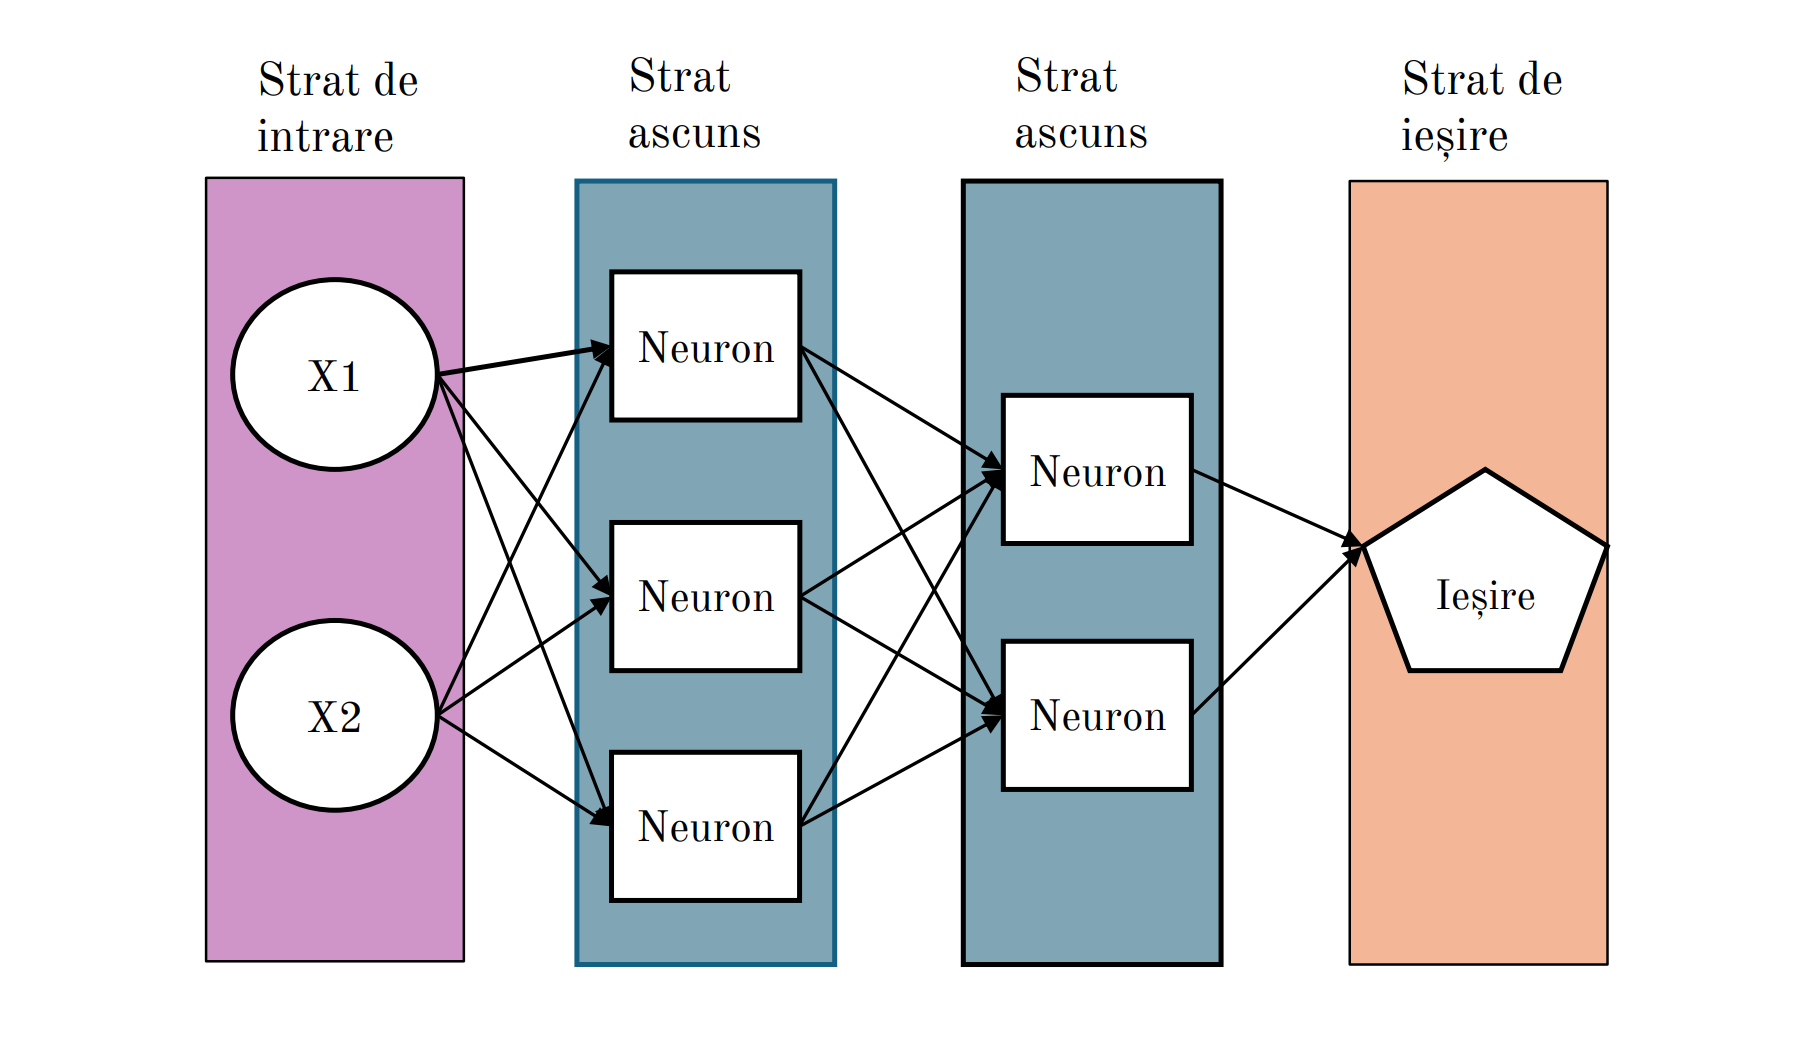
\includegraphics[width=0.9\textwidth]{figuri/retea_neuronala.png}
    \caption{Arhitectura unei rețele neuronale \cite{curs_IA}}
    \label{fig:retea-neuronala}
\end{figure}


    \subsection{Algoritmul de antrenare: Gradient Descent și Backpropagation}

    
Ponderile inițiale ale modelului nu sunt, în general, optime, motiv pentru care se utilizează tehnici de antrenare pentru ajustarea acestora în funcție de setul de date de antrenare.


Scopul unui algoritm de învățare automată este reducerea erorii de generalizare
a modelului. Această eroare reprezintă diferența dintre predicțiile modelului și
valorile reale ale datelor provenite din distribuția reală a fenomenului analizat
și este cunoscută în literatură sub denumirea de risc.

În mod ideal, antrenarea unui model ar presupune minimizarea erorii de predicție pe întreaga distribuție reală a datelor. În practică, însă, această distribuție nu este cunoscută, iar modelul are acces doar la un set finit de exemple de antrenare. Din acest motiv, optimizarea modelului se realizează prin minimizarea erorii medii calculate pe setul de date disponibil, proces cunoscut sub denumirea de minimizare a riscului empiric.

Astfel, în locul riscului real se minimizează riscul empiric, care reprezintă
media erorilor calculate pentru exemplele din setul de antrenare. Procesul de
antrenare bazat pe această idee este cunoscut sub denumirea de \textit{empirical
risk minimization}.

Deși această abordare permite formularea problemei de învățare ca o problemă
de optimizare, ea poate conduce la fenomenul de supraînvățare
(\textit{overfitting}), în special în cazul modelelor cu capacitate mare.
În astfel de situații, modelul poate învăța foarte bine datele de antrenare,
dar performanța sa pe date noi poate fi redusă.

În practica modernă a învățării profunde, optimizarea modelelor se realizează
de obicei prin metode bazate pe algoritmul \textit{gradient descent}, care
permite actualizarea iterativă a parametrilor modelului în direcția reducerii
funcției de pierdere \cite{goodfellow2016}.

Calculul gradientului necesar pentru actualizarea parametrilor unei rețele
neuronale este realizat prin algoritmul \textit{backpropagation}. Acest algoritm
ajustează în mod iterativ ponderile conexiunilor din rețea astfel încât
diferența dintre ieșirea produsă de model și valoarea dorită să fie cât mai mică.
Procesul presupune propagarea erorii de la stratul de ieșire către straturile
anterioare ale rețelei, determinând contribuția fiecărui parametru la eroarea
totală. În urma acestor actualizări, neuronii din straturile ascunse ajung să
reprezinte caracteristici relevante ale datelor, ceea ce permite modelului să
învețe relațiile existente în setul de antrenare \cite{rumelhart1986learning}.


\section{Rețele neuronale recurente (RNN)}
    \subsection{Arhitectura RNN}

Rețelele neuronale recurente (RNN) se numără printre primele arhitecturi dezvoltate pentru procesarea datelor secvențiale, fiind utilizate în aplicații precum modelarea limbajului sau traducerea automată. Un element esențial al acestor rețele este capacitatea de a păstra o stare internă (hidden state), care stochează informații despre intrările anterioare din secvență. Prin intermediul acesteia, RNN-urile pot stoca și modela dependențele temporale existente între elementele secvenței. \cite{dataversity} 

\begin{figure}[H]
\centering

\includegraphics[width=0.9\textwidth]{figuri/RNN.png}
\caption{Arhitectura unei rețele neuronale recurente \cite{jurafsky2023}}
\label{fig:rnn}
\end{figure}

Starea internă a rețelei este actualizată la fiecare pas temporal în funcție de
intrarea curentă și de valoarea stării ascunse din pasul anterior. În acest mod,
ieșirea modelului nu depinde doar de datele curente, ci și de informațiile
procesate anterior. Astfel, rețeaua poate păstra un anumit context al secvenței,
care influențează predicțiile realizate la pașii următori.

Deși introducerea acestei dimensiuni temporale $h_t$ poate face arhitectura să pară
mai complexă decât rețelele neuronale clasice de tip feedforward, mecanismul
de calcul rămâne similar. La fiecare pas temporal, modelul primește vectorul
de intrare și starea ascunsă din momentul precedent, iar pe baza acestora
calculează noua stare internă a rețelei. Conexiunile recurente dintre stările
ascunse permit modelului să utilizeze informațiile din trecut pentru a produce
ieșirea corespunzătoare intrării curente \cite{jurafsky2023}.

\begin{figure}[h]
    \centering
    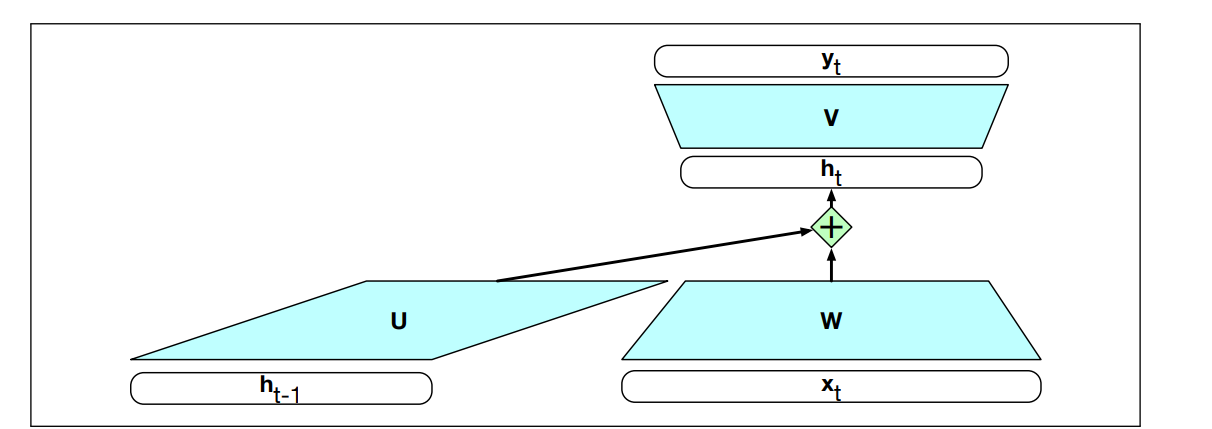
\includegraphics[width=0.9\textwidth]{figuri/RNN_desfasurat.png}
    \caption{Arhitectura RNN desfășurată \cite{jurafsky2023}}
    \label{fig:rnn-desfasurat}
\end{figure}


    \subsection{Limitări ale RNN}

Antrenarea rețelelor neuronale recurente poate fi dificilă
în cazul aplicațiilor care necesită utilizarea unor informații aflate la
o distanță mare în cadrul secvenței. Deși, teoretic, RNN-urile au acces
la întreaga secvență anterioară, informația codificată în stările ascunse
tinde să fie mai degrabă locală, fiind mai relevantă pentru cele mai
recente elemente ale secvenței și pentru deciziile luate recent.

În mod ideal, o rețea ar trebui să fie capabilă să păstreze informații
aflate la distanță în secvență până în momentul în care acestea devin
relevante, procesând în același timp corect elementele intermediare.
În practică însă, straturile ascunse și ponderile asociate acestora sunt
nevoite să îndeplinească simultan două roluri: să furnizeze informații
utile pentru decizia curentă și, în același timp, să actualizeze și să
transmită mai departe informațiile necesare pentru deciziile viitoare.

O altă dificultate apare în timpul procesului de antrenare, atunci când eroarea trebuie propagată înapoi prin mai mulți pași temporali.
În această situație, gradientul funcției cost este supus unor multiplicări
repetate, determinate de lungimea secvenței. Ca urmare, valorile
gradientului pot scădea progresiv până aproape de zero, fenomen
cunoscut sub denumirea de \textit{vanishing gradient}. 
        \subsubsection{Problema vanishing gradient}

Această problemă apare în special în cazul rețelelor neuronale recurente, unde procesul de antrenare implică propagarea erorii prin mai mulți pași temporali. În timpul
\textit{backpropagation through time}, gradientul este multiplicat
în mod repetat cu aceleași ponderi ale rețelei. Dacă valorile acestor
ponderi sunt mici, gradientul poate scădea rapid spre zero,
ceea ce face dificilă actualizarea eficientă a parametrilor
rețelei pentru informații aflate la distanță în secvență. \cite{jurafsky2023}
    \subsection{Modele îmbunătățite: LSTM și GRU}

Pentru a depăși limitările rețelelor neuronale recurente clasice, au fost
propuse arhitecturi mai complexe, dintre care cea mai utilizată este
\textit{Long Short-Term Memory} (LSTM), introdusă de Hochreiter și
Schmidhuber, în 1997 \cite{hochreiter1997long}. Rețelele LSTM abordează
problema gestionării contextului prin separarea a două procese
esențiale: eliminarea informațiilor care nu mai sunt relevante și
păstrarea informațiilor utile pentru deciziile ulterioare. Spre
deosebire de arhitecturile RNN clasice, în care modul de gestionare a
contextului este implicit, LSTM permite rețelei să învețe automat cum
să controleze fluxul informației de-a lungul secvenței.

Pentru a realiza acest lucru, LSTM utilizează unități neuronale
specializate care includ mecanisme de tip \textit{gates} (porți),
responsabile pentru controlul fluxului de informație care intră și
iese din celula de memorie.

Porțile (\textit{gates}) dintr-o rețea LSTM au rolul de a controla
fluxul de informație în cadrul celulei de memorie. Fiecare poartă
utilizează un strat de tip \textit{feedforward} urmat de o funcție de
activare sigmoid, care produce valori cuprinse între 0 și 1. Aceste
valori determină în ce măsură informația este transmisă mai departe
sau eliminată, permițând rețelei să păstreze doar informațiile
relevante pentru procesarea ulterioară.

\begin{figure}[h]
    \centering
    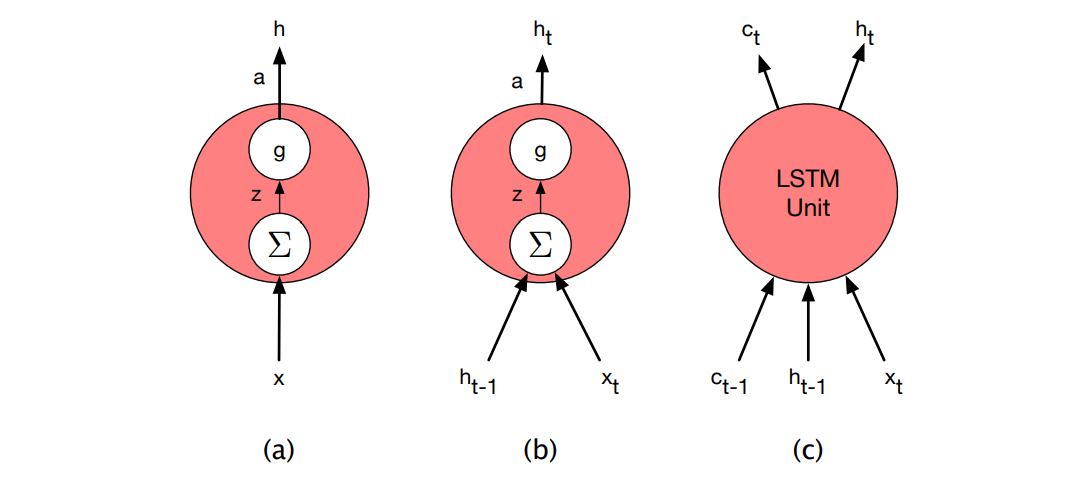
\includegraphics[width=0.9\textwidth]{figuri/Comparatie structura.png}
\caption{Arhitectura neuronului utilizat în rețele feedforward,
Rețele Neuronale Recurente (RNN) și rețele Long Short-Term Memory (LSTM) \cite{jurafsky2023}}
    \label{fig:comparatie-rnn-lstm}
\end{figure}

\section{Arhitectura Transformer}

Termenul Transformer a fost introdus pentru prima dată în articolul „Attention Is All You Need” \cite{vaswani2017attention} publicat în 2017 de către Vaswani și colaboratorii săi, în care autorii propun un model bazat exclusiv pe mecanismul de self-attention pentru procesarea secvențelor, fără utilizarea
recurenței specifice rețelelor neuronale recurente. Spre deosebire de arhitecturile bazate pe rețele neuronale recurente, care procesează datele în mod secvențial, modelul Transformer permite analizarea simultană a tuturor elementelor unei secvențe. Această abordare facilitează paralelizarea calculelor și permite capturarea
dependențelor dintre elemente aflate la distanță în secvență.

    \subsection{Structura encoder–decoder}

La baza Transformerelor stă o arhitectură de tip encoder-decoder. Acest tip de arhitectură este utilizat pentru a transforma o secvență de intrare într-o secvență de ieșire, fiind frecvent întâlnită în aplicații precum traducerea automată \cite{sutskever2014sequence}.


Modelul este alcătuit din două componente principale. Encoderul primește secvența de intrare și o procesează element cu element, construind treptat o reprezentare internă a acesteia. La finalul procesării, informația este sintetizată într-un vector de context, care conține informația esențială despre întreaga secvență de intrare.

Acest vector de context este transmis către decoder, care generează secvența de ieșire pas cu pas. La fiecare pas, decoderul utilizează atât informația din vectorul de context, cât și elementele generate anterior, pentru a produce următorul element din secvență.
Un avantaj important al acestei arhitecturi este flexibilitatea în ceea ce privește lungimea secvențelor: numărul de elemente din intrare poate fi diferit de cel din ieșire. Encoderul și decoderul sunt antrenate împreună, astfel încât modelul să învețe relația dintre secvențele de intrare și cele de ieșire \cite{goodfellow2016}.

Totuși, în variantele clasice bazate pe rețele neuronale recurente, întreaga informație a secvenței de intrare este comprimată într-un singur vector de context. Această limitare poate duce la pierderi de informație, în special în cazul secvențelor lungi, deoarece modelul nu poate păstra eficient toate detaliile relevante.

Pentru a rezolva această problemă, au fost introduse ulterior mecanisme de tip attention, care permit modelului să acceseze direct diferite părți ale secvenței de intrare în timpul generării rezultatului \cite{bahdanau2015neural}.
\begin{figure}[H]
    \centering
    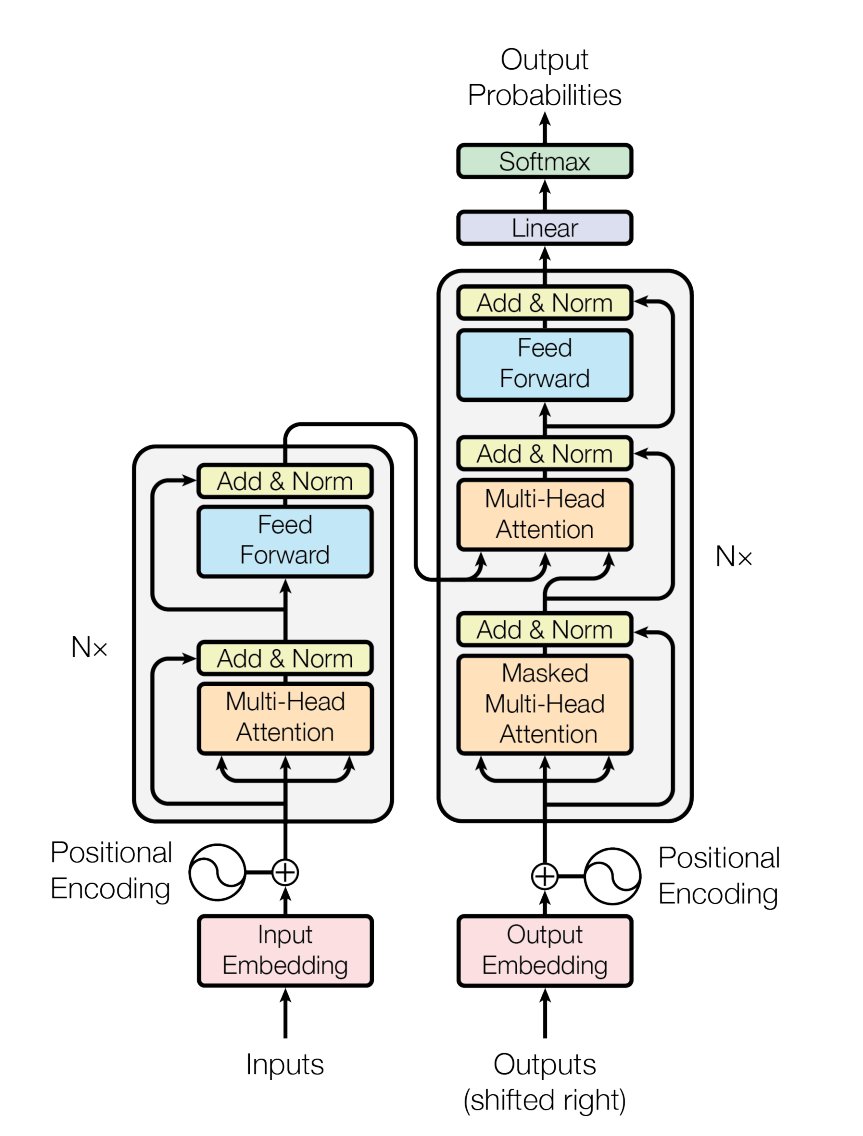
\includegraphics[width=0.8\textwidth]{figuri/encoder_decoder_ai.png}
    \caption{Arhitectura encoder-decoder \cite{vaswani2017attention}}
\end{figure}

    \subsection{Mecanismul self-attention}
    
Mecanismul de \textit{attention} poate fi privit ca un mod prin care
modelul decide asupra căror elemente din secvență trebuie să se
concentreze. Acesta primește o interogare (\textit{query}) și un set
de perechi cheie–valoare (\textit{key–value}), iar rezultatul este
obținut prin combinarea valorilor în funcție de cât de relevante sunt
pentru interogarea respectivă. Gradul de relevanță este determinat
prin compararea interogării cu fiecare cheie din secvență. 

Scorul de relevanță dintre query și fiecare key este calculat printr-o funcție de similaritate, de obicei produs scalar (dot-product), urmat de o normalizare cu funcția softmax.

Prin acest mecanism, modelul nu mai este limitat la un singur vector de context, ci poate accesa direct informații din întreaga secvență de intrare, ceea ce permite captarea mai eficientă a dependențelor pe termen lung \cite{vaswani2017attention}.
    
\section{Modele bazate pe Transformer}

Datorită capacității de a procesa secvențe în paralel și de a capta dependențe pe termen lung, arhitectura Transformer descrisă în secțiunea anterioară stă la baza celor mai performante modele actuale de procesare a limbajului natural \cite{datacamp}.

    \subsection{Modele lingvistice de mari dimensiuni (LLM)}

Modelele lingvistice de mari dimensiuni (LLM) reprezintă o categorie de modele de limbaj bazate pe rețele neuronale cu un număr foarte mare de parametri, antrenate pe volume extinse de date textuale neetichetate prin tehnici de învățare auto-supervizată \cite{brown2020language}. Prin pre-antrenarea pe corpusuri de mari dimensiuni, aceste modele dobândesc capacitatea de a identifica tipare complexe, nuanțe semantice și relații contextuale în limbajul natural, putând fi utilizate pentru generarea de text, traducerea automată, sumarizarea documentelor, răspunsul la întrebări sau analiza sentimentelor. Adaptarea lor pentru sarcini specifice prin tehnici de fine-tuning a condus la performanțe de ultimă generație în numeroase aplicații. 

\begin{figure}[H]
    \centering
    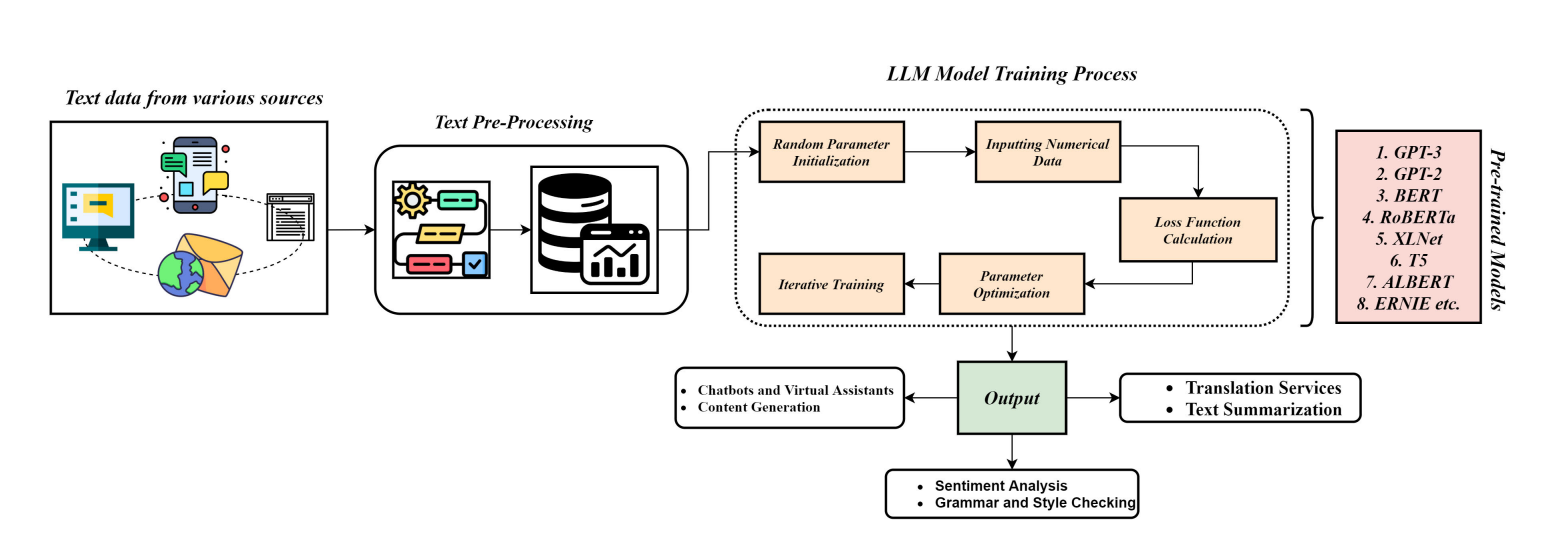
\includegraphics[width=\textwidth]{figuri/antrenare_llm.png}
    \caption{Procesul de antrenare al modelelor LLM \cite{llm_review_2024}}
    
\end{figure}

Arhitectura modelelor lingvistice de mari dimensiuni (LLM) presupune preluarea datelor text din multiple surse, urmată de transmiterea acestora către etapele de preprocesare. Procesul de antrenare include mai multe etape, precum inițializarea aleatorie a parametrilor, transformarea datelor în format numeric, calculul funcției de pierdere, optimizarea parametrilor și antrenarea iterativă a modelului.

După finalizarea antrenării, aceste modele pot fi utilizate pentru diverse sarcini de procesare a limbajului natural.

Odată cu dezvoltarea unor modele avansate, precum GPT, LLaMA sau Bard, și explorarea capacităților acestora în diverse aplicații, LLM-urile au devenit un domeniu esențial și extrem de activ în cercetarea actuală. În acest context, evaluarea performanței și a fiabilității acestor modele reprezintă o direcție importantă de studiu. \cite{llm_review_2024}.


    \subsection{Procesul de antrenare al modelelor LLM}
După cum se observă în figura 1.7, antrenarea LLM se poate împărți în mai mulți pași. După filtrarea datelor, 
tokenizarea reprezintă una dintre etapele esențiale de preprocesare în cadrul modelelor lingvistice de mari dimensiuni. Aceasta constă în împărțirea textului în unități discrete, denumite tokeni, care pot fi caractere, subcuvinte, simboluri sau cuvinte, în funcție de tipul modelului utilizat. În practică, sunt folosiți diverși algoritmi de tokenizare, precum WordPiece, UnigramLM sau Byte Pair Encoding (BPE), fiecare având o metodă specifică de segmentare a textului de intrare.

\begin{figure}[H]
    \centering
    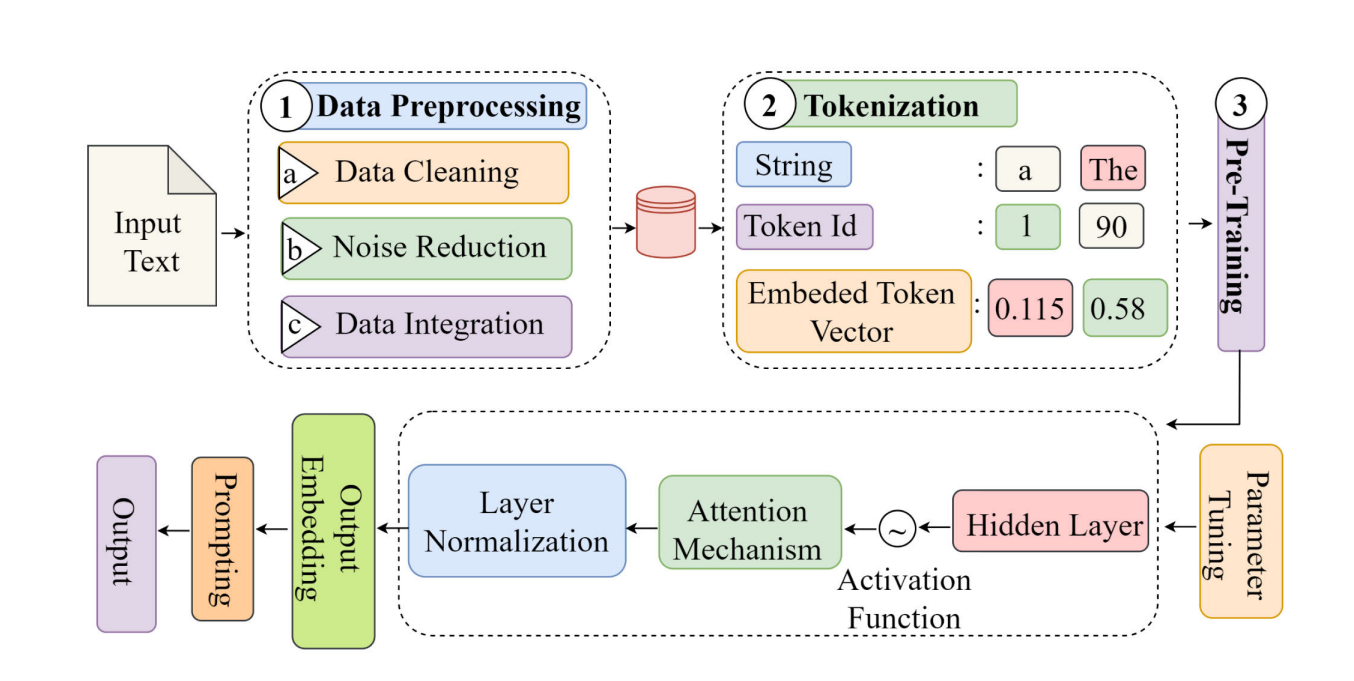
\includegraphics[width=0.8\textwidth]{figuri/LLM_stages.png}
    \caption{Pipeline complet LLM \cite{llm_review_2024}}
    
\end{figure}

După etapa de preprocesare, datele sunt transformate într-o formă numerică și utilizate în procesul de antrenare al modelului. Acesta include inițializarea parametrilor, calculul funcției de pierdere, optimizarea parametrilor și antrenarea iterativă, până la convergența modelului. Prin acest proces, modelul învață să identifice tipare și relații complexe în limbajul natural.

\section{Retrieval-Augmented Generation (RAG)}

Modelele lingvistice de mari dimensiuni pre-antrenate au demonstrat capacitatea de a stoca cunoștințe factuale în parametrii lor și de a obține performanțe ridicate atunci când sunt adaptate (fine-tuned) pentru sarcini specifice de procesare a limbajului natural. Cu toate acestea, capacitatea lor de a accesa și de a utiliza în mod precis aceste cunoștințe este limitată, ceea ce conduce la performanțe inferioare în cazul sarcinilor care necesită informații detaliate și actualizate.

De asemenea, dificultatea de a furniza surse clare pentru informațiile generate, precum și de a actualiza cunoștințele interne ale modelului, reprezintă provocări importante în utilizarea acestor modele, motiv pentru care au fost propuse abordări care integrează mecanisme de acces la surse externe de informație prin utilizarea unei memorii non-parametrice \cite{lewis2020retrieval}.



\subsection{Conceptul de Retrieval-Augmented Generation}

O astfel de abordare este reprezentată de modelele de tip Retrieval-Augmented Generation (RAG), care combină memoria parametrică a modelului, învățată în timpul antrenării, cu o memorie non-parametrică externă, bazată pe regăsirea documentelor relevante \cite{lewis2020retrieval}. În lucrarea originală, această memorie externă este implementată ca un index vectorial dens de documente, accesat printr-un mecanism de regăsire neurală.

În această paradigmă, modelul nu se bazează exclusiv pe cunoștințele stocate în parametrii săi, ci utilizează documentele recuperate ca sursă suplimentară de context în procesul de generare a răspunsului. Pentru sarcini intensive în cunoștințe, această arhitectură permite generarea unor răspunsuri mai specifice și mai factuale decât în cazul modelelor bazate exclusiv pe memorie parametrică \cite{lewis2020retrieval}.

Această abordare contribuie la îmbunătățirea performanței în sarcini care necesită acces la cunoștințe detaliate sau actualizate și reduce riscul de generare a unor informații eronate, fenomen cunoscut sub denumirea de halucinații. În plus, RAG permite separarea cunoștințelor de model de datele utilizate, facilitând actualizarea informațiilor fără a fi necesară reantrenarea completă a modelului.

Prin integrarea mecanismelor de regăsire și generare, modelele RAG oferă un cadru flexibil pentru rezolvarea sarcinilor de procesare a limbajului natural, în special în aplicații care necesită acces la baze de cunoștințe extinse \cite{lewis2020retrieval} sau la proceduri interne.


\subsection{Arhitectura Retrieval-Augmented Generation}

Arhitectura modelelor de tip Retrieval-Augmented Generation este construită în jurul interacțiunii dintre două componente principale: un mecanism de regăsire a documentelor și un model de generare, integrate într-un cadru probabilistic unificat \cite{lewis2020retrieval}.

Componenta de regăsire, bazată pe Dense Passage Retriever (DPR), are rolul de a identifica un set de documente relevante în raport cu secvența de intrare. Atât interogările, cât și documentele sunt proiectate numeric într-un spațiu vectorial comun, iar selecția se realizează pe baza similarității, utilizând o aproximare de tip top-K. Documentele astfel obținute sunt tratate ca variabile latente în cadrul modelului.

Componenta de generare este reprezentată de un model de tip sequence-to-sequence bazat pe Transformer, precum BART sau T5, care utilizează atât secvența de intrare, cât și documentele recuperate pentru a genera răspunsul final. Generarea este condiționată de aceste documente, iar contribuția fiecăruia este integrată prin marginalizare asupra variabilelor latente.

În practică, această integrare se realizează printr-o aproximare top-K, care poate fi aplicată fie la nivelul întregii secvențe generate, fie la nivelul fiecărui token. În primul caz, se presupune că același document este responsabil pentru întreaga secvență de ieșire, în timp ce, în al doilea caz, diferite documente pot contribui la generarea fiecărui token.

Un aspect esențial al acestei arhitecturi îl reprezintă antrenarea comună a componentelor de regăsire și generare, într-un mod end-to-end. Această strategie permite optimizarea simultană a selecției documentelor și a procesului de generare, astfel încât informațiile recuperate să fie cât mai relevante pentru răspunsul final.

Prin utilizarea documentelor externe ca sursă de context, arhitectura RAG permite modelului să acceseze informații suplimentare în timpul inferenței, fără a depinde exclusiv de cunoștințele stocate în parametrii săi \cite{lewis2020retrieval}.

\begin{figure}[H]
    \centering
    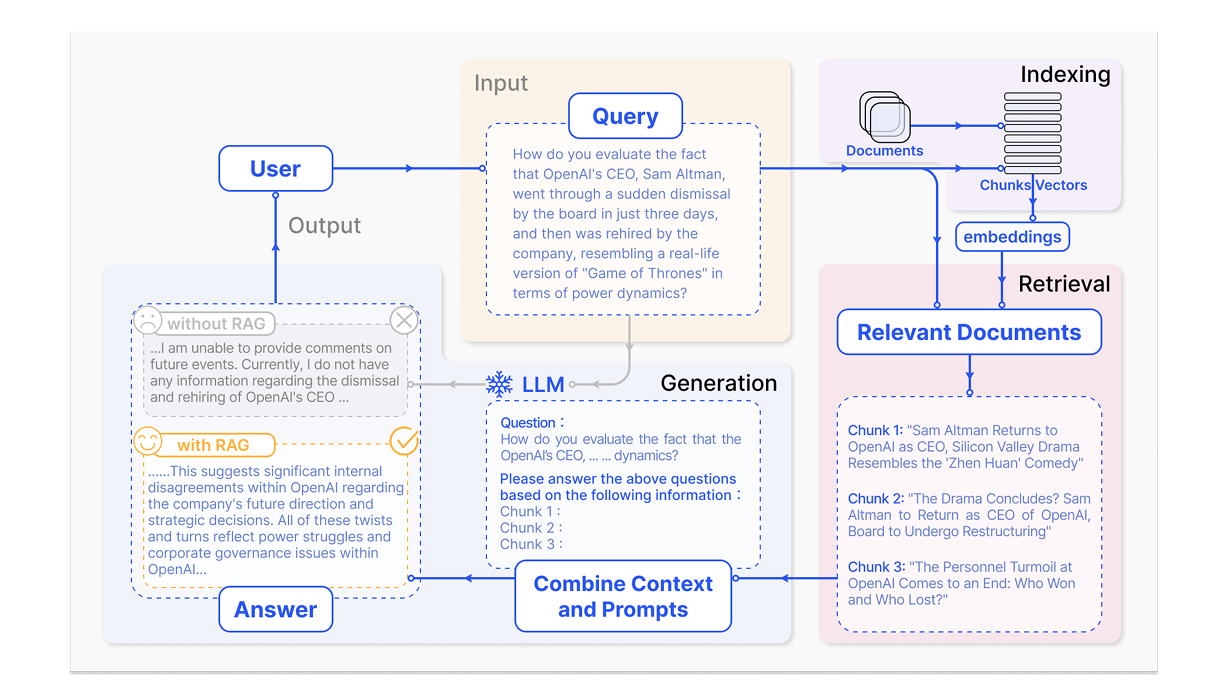
\includegraphics[width=\textwidth]{figuri/rag_arch.png}
    \caption{Arhitectura modelului RAG \cite{gao2023retrieval}}
    
\end{figure}

\subsection{Măsurarea similarității}
\label{sec:similaritate}

Atât interogarea utilizatorului, cât și fragmentele de text extrase din documente sunt transformate în reprezentări numerice, denumite embeddings. Acestea sunt proiectate într-un spațiu vectorial, în care se evaluează gradul de similaritate semantică dintre interogare și fiecare fragment de text.

Similaritatea sau distanța dintre aceste reprezentări poate fi calculată utilizând diferite măsuri, alegerea acestora reprezentând un hiperparametru al sistemului. Cele mai utilizate metode includ similaritatea cosinus, produsul scalar, distanța euclidiană și distanța Manhattan.

\begin{figure}[H]
    \centering
    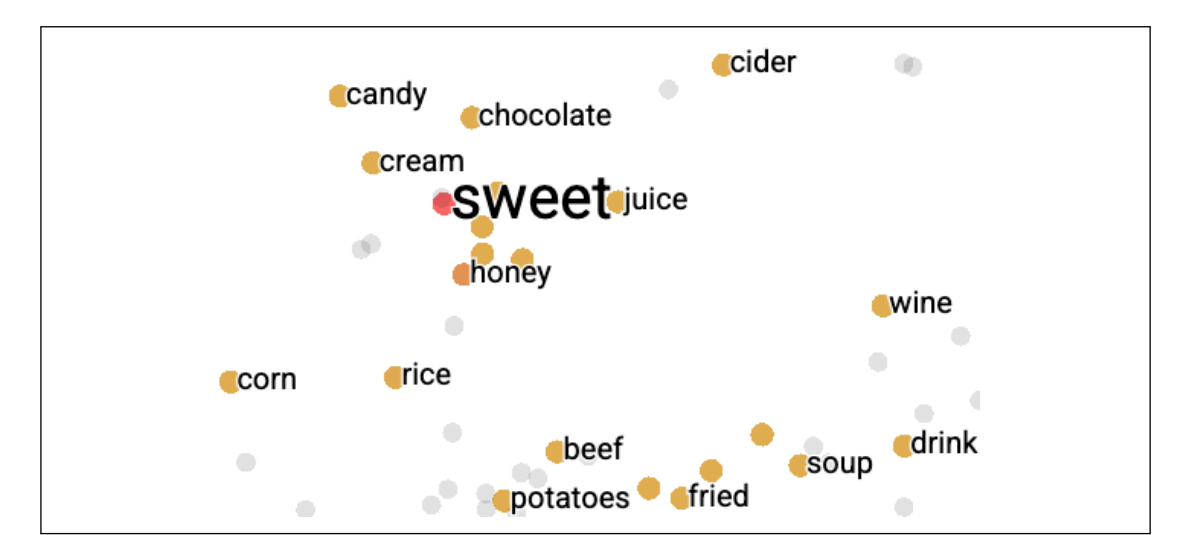
\includegraphics[width= 0.8\textwidth]{figuri/Distance.png}
    \caption{Vizualizarea în 2D a embedding-urilor Word2Vec, evidențiind gruparea semantică a cuvintelor similare (adaptat după \cite{mikolov2013word2vec})}
    
\end{figure}

\begin{itemize}
    \item \textbf{Similaritatea cosinus} măsoară unghiul dintre doi vectori în spațiul vectorial, fiind definită ca:

\begin{equation}
\text{sim}_{cos}(P, Q) = \frac{P \cdot Q}{\|P\| \|Q\|}
\end{equation}

Valorile apropiate de 1 indică similaritate semantică ridicată, cele apropiate de 0 — similaritate redusă, iar valorile negative semnalează o orientare opusă. Uneori se preferă distanța cosinus, complementul față de 1 al similarității:

\begin{equation}
d_{cos}(P, Q) = 1 - \text{sim}_{cos}(P, Q)
\end{equation}

    \item \textbf{Distanța euclidiană} ($L_2$) cuantifică distanța geometrică directă dintre doi vectori, derivată din teorema lui Pitagora:

\begin{equation}
d_{L_2}(P, Q) = \sqrt{\sum_{i=1}^{d} (P_i - Q_i)^2}
\end{equation}

Cu cât valoarea este mai mică, cu atât similaritatea dintre reprezentări este mai ridicată.

    \item \textbf{Distanța Manhattan} ($L_1$) calculează suma diferențelor absolute ale componentelor, modelând deplasarea restricționată la direcții ortogonale — analogă navigației pe o rețea stradală:

\begin{equation}
d_{L_1}(P, Q) = \sum_{i=1}^{d} |P_i - Q_i|
\end{equation}

    \item \textbf{Produsul scalar} exprimă similaritatea ca sumă a produselor componentelor corespunzătoare:

\begin{equation}
P \cdot Q = \sum_{i=1}^{d} P_i Q_i
\end{equation}

Spre deosebire de similaritatea cosinus, rezultatul depinde atât de direcția, cât și de magnitudinea vectorilor, ceea ce îl face util în scenarii unde amplitudinea reprezentărilor este relevantă. \cite{levy2024similarity}

\end{itemize}
\subsection{Avantaje și limitări ale RAG}

Modelele de tip Retrieval-Augmented Generation oferă avantaje semnificative față de
modelele lingvistice clasice. Principalul beneficiu constă în capacitatea de a accesa
informații externe în timpul inferenței, ceea ce reduce riscul de generare a unor
afirmații factuale eronate și permite producerea unor răspunsuri mai bine fundamentate
în sarcinile ce necesită cunoștințe detaliate sau actualizate.

Un alt avantaj important îl reprezintă separarea memoriei parametrice de cea
non-parametrică: informațiile pot fi actualizate prin modificarea bazei de documente,
fără a fi necesară reantrenarea modelului. Aceasta conferă sistemelor RAG o
flexibilitate ridicată în contexte cu date în continuă schimbare. \cite{lewis2020retrieval}

Cu toate acestea, arhitectura RAG introduce și o serie de limitări. Performanța
sistemului depinde direct de calitatea componentei de regăsire: documentele
nerelevante selectate propagă erori în răspunsul final. Totodată, modul în care
textul sursă este fragmentat influențează semnificativ relevanța rezultatelor —
o segmentare necorespunzătoare poate conduce la pierderea contextului semantic
sau la recuperarea unor informații incomplete \cite{gao2023retrieval}. În plus,
integrarea etapei de regăsire introduce un cost computațional suplimentar față
de modelele generative clasice, crescând latența sistemului.

\section{Modele agentice și extinderea RAG}

Integrarea mecanismelor agentice în sistemele bazate pe Retrieval-Augmented Generation 
extinde fluxul clasic RAG, în care documentele relevante sunt recuperate și utilizate 
drept context pentru generarea răspunsului \cite{lewis2020retrieval}. Într-o arhitectură 
agentică, acest flux poate fi completat cu etape explicite de planificare, decizie și 
acțiune, specifice sistemelor autonome bazate pe LLM \cite{wang2024survey}. Astfel, 
sistemul poate selecta dinamic pașii de procesare, poate rafina interogările și poate 
adapta strategia de răspuns în funcție de obiectivul urmărit.

Agentic AI desemnează o clasă de sisteme de inteligență artificială capabile să acționeze 
autonom pentru atingerea unor obiective complexe, cu supraveghere umană minimă. Aceste 
sisteme combină capacitățile generative ale modelelor lingvistice de mari dimensiuni (LLM) 
cu mecanisme de planificare, utilizare a instrumentelor externe și adaptare la feedback-ul 
din mediul de execuție. \cite{ibm_agentic}

\begin{figure}[H]
    \centering
    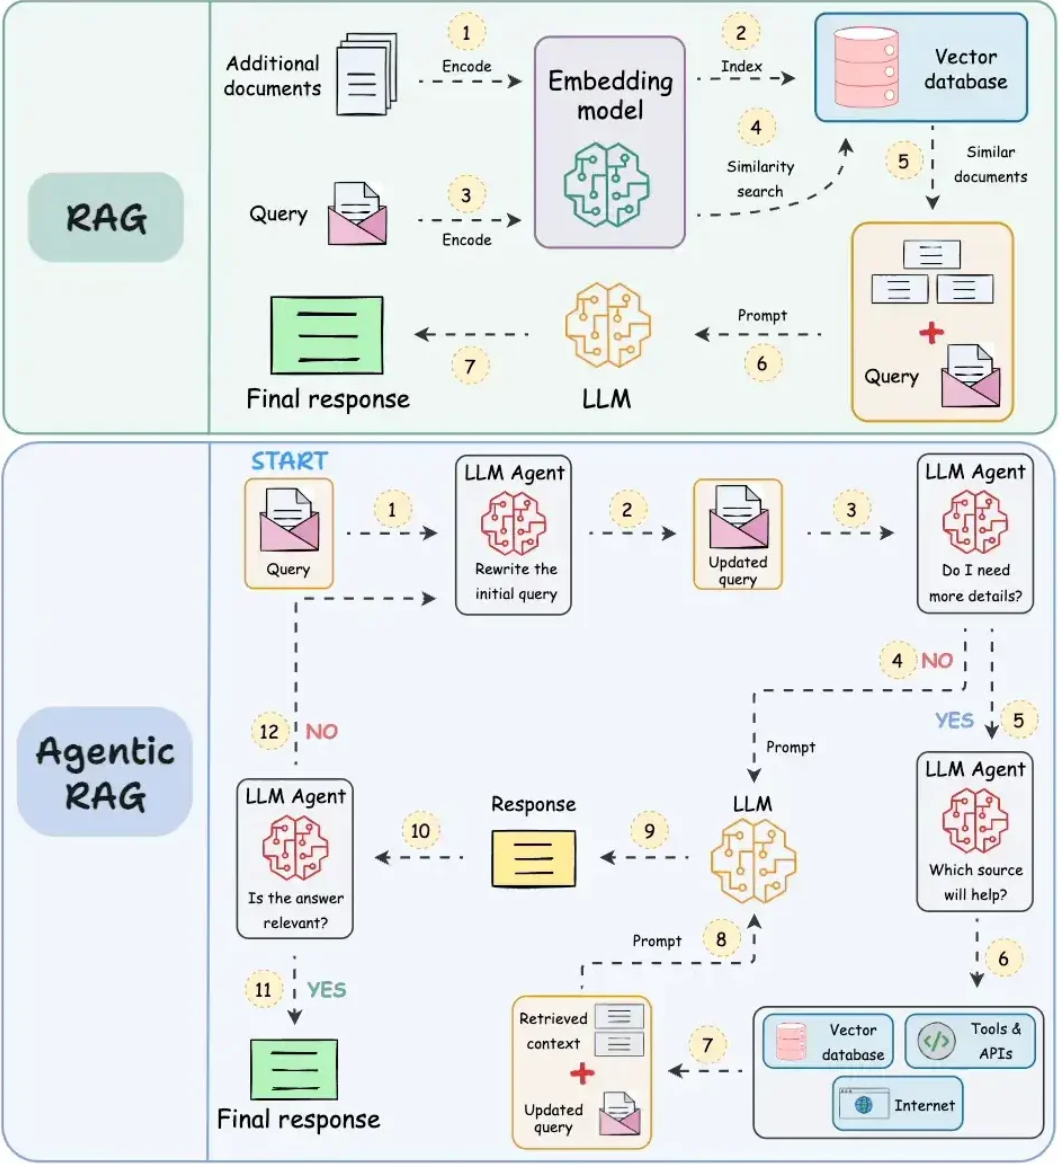
\includegraphics[width=0.8\textwidth]{figuri/agentic.png}
    \caption{Arhitectura unui sistem Agentic AI \cite{dextralabs}}
\end{figure}

\subsection{Generative AI vs Agentic AI}

Distincția dintre sistemele generative și cele agentice poate fi surprinsă prin modul 
în care fiecare categorie se raportează la sarcini și la interacțiunea cu mediul.

Modelele generative clasice (Generative AI) operează reactiv: primesc o intrare de la 
utilizator și produc un răspuns într-un singur pas de inferență, fără a putea planifica 
acțiuni ulterioare sau a interacționa cu surse externe. Capacitățile lor sunt limitate 
la cunoștințele dobândite în etapa de antrenare.

Sistemele agentice (Agentic AI), în schimb, adoptă o abordare proactivă și iterativă. 
Acestea sunt capabile să descompună un obiectiv complex în subobiective, să selecteze 
și să invoce instrumente externe (baze de date, API-uri, motoare de căutare), să 
evalueze rezultatele intermediare și să își ajusteze planul de acțiune în consecință. 
Acest ciclu de percepție–raționament–acțiune le conferă un grad de autonomie 
calitativ superior față de modelele generative tradiționale. \cite{wang2024survey}

\begin{table}[H]
\centering
\renewcommand{\arraystretch}{1.4}
\begin{tabular}{|p{3.5cm}|p{5cm}|p{5cm}|}
\hline
\textbf{Criteriu} & \textbf{Generative AI} & \textbf{Agentic AI} \\
\hline
Mod de operare & Reactiv — generează un răspuns la o intrare dată & Proactiv — planifică și execută acțiuni pentru atingerea unui obiectiv \\
\hline
Memorie & Limitată la fereastra de context curentă & Persistentă — poate stoca și accesa informații între sesiuni \\
\hline
Acces la resurse externe & Nu interacționează cu surse externe & Poate invoca API-uri, baze de date, motoare de căutare \\
\hline
Planificare & Absentă — răspunde într-un singur pas de inferență & Prezentă — descompune obiective complexe în subobiective \\
\hline
Autonomie & Redusă — necesită intervenție umană la fiecare pas & Ridicată — poate acționa cu supraveghere minimă \\
\hline
Adaptabilitate & Statică față de mediul de execuție & Dinamică — ajustează comportamentul pe baza feedback-ului \\
\hline
Caz de utilizare tipic & Generare de text, rezumare, traducere & Automatizare de fluxuri complexe, agenți de cercetare \\
\hline
\end{tabular}
\caption{Comparație între sistemele Generative AI și Agentic AI}
\label{tab:gen_vs_agentic}
\end{table}



\cleardoublepage
\chapter{Prezentarea tehnologiilor folosite}

\begin{table}[h]
\centering
\caption{Rolul principalelor tehnologii utilizate în proiect}
\begin{tabular}{|p{3cm}|p{4cm}|p{6cm}|}
\hline
\textbf{Tehnologie} & \textbf{Categorie} & \textbf{Rol în proiect} \\
\hline
Python & Limbaj de programare & Implementarea logicii aplicației, a modulelor RAG, guardrails, evaluare și orchestrare \\
\hline
Flask & Framework web & Expunerea endpoint-urilor REST și compatibilitatea cu clienți conversaționali \\
\hline
Qdrant & Bază de date vectorială & Stocarea embedding-urilor și regăsirea semantică a fragmentelor relevante \\
\hline
LlamaIndex & Framework RAG & Segmentarea semantică a documentelor și integrarea cu fluxul de indexare \\
\hline
Kuzu & Bază de date grafică & Reprezentarea entităților medicale și a relațiilor dintre acestea \\
\hline
OpenAI / Anthropic / Ollama & Furnizori LLM & Generarea răspunsurilor prin modele cloud sau locale \\
\hline
Docker Compose & Orchestrare containere & Pornirea coordonată a serviciilor aplicației \\
\hline
unittest / coverage.py & Testare & Validarea componentelor și măsurarea acoperirii testelor \\
\hline
\end{tabular}
\end{table}

\section{Limbajul de programare}

Python reprezintă limbajul de programare ales pentru implementarea acestui sistem,
datorită ecosistemului extins de biblioteci specializate în domeniul inteligenței
artificiale și al procesării limbajului natural \cite{srinath2017python, llm_review_2024}. În contextul unui
chatbot medical bazat pe o arhitectură RAG augmentată cu un knowledge graph,
Python oferă integrări native cu principalele framework-uri relevante: biblioteca
\texttt{llama-index} asigură orchestrarea pipeline-ului de regăsire și generare,
\texttt{kuzu} gestionează stocarea și interogarea grafului de cunoștințe medicale
ca bază de date graf autonomă, eliminând necesitatea unui server dedicat, iar
\texttt{openai} și \texttt{anthropic} permit integrarea furnizorilor de servicii
LLM fără efort suplimentar de integrare. Suportul extins pentru procesarea
documentelor, gestionarea datelor tabelare și apelurile HTTP asincrone permite
construirea unui pipeline de ingestie complet fără a recurge la limbaje auxiliare.

Implementarea utilizează Python 3.11, versiune care aduce îmbunătățiri măsurabile
de performanță față de versiunile anterioare — cu până la 60\% mai rapid în anumite
scenarii de execuție, conform documentației oficiale \cite{python311} — precum și
mesaje de eroare semnificativ îmbunătățite, care facilitează depanarea pipeline-ului
de procesare. Utilizarea instrumentelor standardizate pentru gestionarea mediilor
virtuale, precum \texttt{venv}, simplifică reproducerea exactă
a configurației software și reduce riscul incompatibilităților între versiunile
bibliotecilor.



\section{Interfața API}


\subsection{Interfața REST}

În cadrul aplicațiilor software moderne, comunicarea dintre componente diferite ale unui sistem este realizată frecvent prin intermediul unor interfețe de programare a aplicațiilor, cunoscute sub denumirea de API-uri. În cazul aplicațiilor web, această comunicare este realizată prin protocolul HTTP, unde un client trimite o cerere către un server, iar serverul procesează cererea și returnează un răspuns \cite{mdn_client_server}. Acest model este potrivit pentru sisteme în care interfața de utilizare, logica aplicației și serviciile externe trebuie să comunice printr-un mecanism standardizat.

REST, acronim pentru \textit{Representational State Transfer}, reprezintă un stil arhitectural pentru sisteme distribuite de tip hypermedia, definit de Roy Fielding în teza sa de doctorat \cite{fielding_rest}. Arhitectura REST este organizată în jurul conceptului de resursă, iar interacțiunea dintre componente se realizează prin transferul reprezentărilor acestor resurse. Fiecare resursă poate fi identificată printr-un URI, iar operațiile asupra acesteia sunt realizate prin metode HTTP standard \cite{fielding_rest,mdn_rest}.

Un principiu important al REST este separarea dintre client și server. În această abordare, clientul este responsabil de inițierea cererilor și de prezentarea informațiilor către utilizator, în timp ce serverul gestionează procesarea cererilor și furnizarea răspunsurilor. Această separare permite dezvoltarea independentă a componentelor, atât timp cât interfața de comunicare rămâne stabilă \cite{fielding_rest}.

O altă caracteristică esențială este comunicarea fără stare, numită \textit{stateless}. În arhitectura REST, fiecare cerere transmisă de client trebuie să conțină toate informațiile necesare pentru ca serverul să o poată procesa, fără ca serverul să depindă de contextul unei cereri anterioare \cite{fielding_rest}. Această idee este compatibilă și cu natura protocolului HTTP, care nu păstrează în mod implicit informații despre comunicări anterioare între client și server \cite{mdn_http}.

În practică, interacțiunea cu o interfață REST este realizată prin metode HTTP. Metoda \texttt{GET} este utilizată pentru solicitarea unei reprezentări a unei resurse, metoda \texttt{POST} pentru transmiterea unor date către server, metoda \texttt{PUT} pentru crearea sau înlocuirea unei resurse, iar metoda \texttt{DELETE} pentru solicitarea ștergerii unei resurse \cite{mdn_http_methods}. Astfel, operațiile efectuate asupra datelor sunt exprimate prin mecanisme HTTP standard, ceea ce face interfața mai ușor de înțeles și de integrat cu alte aplicații.

În proiectul dezvoltat, interfața REST are rolul de a expune funcționalitățile backend-ului către alte aplicații sau interfețe externe. Prin intermediul acesteia, un client poate trimite o cerere către sistem, iar backend-ul returnează un răspuns structurat. În cazul aplicației realizate, fluxul presupune primirea unei cereri HTTP, extragerea datelor transmise de client, apelarea componentelor interne ale sistemului și returnarea rezultatului către client. Această organizare respectă principiul separării dintre interfața de acces și logica internă a aplicației, principiu asociat arhitecturii client-server din REST \cite{fielding_rest}.


\subsection{Framework-ul Flask}


Pentru implementarea acestei interfețe a fost utilizat framework-ul Flask. Flask este un framework web WSGI pentru limbajul Python, proiectat pentru dezvoltarea rapidă a aplicațiilor web și pentru extinderea acestora către proiecte mai complexe \cite{flask_doc}. Această caracteristică îl face potrivit pentru proiecte modulare, în care dezvoltatorul dorește să definească explicit rutele aplicației și modul în care sunt tratate cererile HTTP.

Un avantaj al Flask este faptul că permite definirea directă a rutelor prin funcții Python. Astfel, o adresă URL poate fi asociată cu o funcție care primește cererea, procesează datele și returnează răspunsul corespunzător. În contextul proiectului, Flask este utilizat ca strat de comunicare între interfața externă și componentele interne ale sistemului. Acesta preia cererile HTTP, extrage conținutul transmis de client, apelează modulul responsabil de procesarea mesajului și returnează rezultatul într-un format standardizat.

Prin utilizarea unei interfețe REST implementate cu Flask, sistemul obține o structură clară și ușor de integrat. REST oferă modelul arhitectural pentru comunicarea dintre client și server, iar Flask oferă mecanismele practice prin care acest model poate fi implementat în Python. Această combinație este potrivită pentru aplicații academice și prototipuri funcționale, deoarece permite expunerea rapidă a funcționalităților backend-ului printr-un API accesibil altor componente software.

\subsection{Interfața OpenWebUI}

OpenWebUI este o platformă web open-source, self-hosted, utilizată pentru interacțiunea cu sisteme bazate pe inteligență artificială printr-o interfață grafică. Platforma este prezentată ca fiind extensibilă, bogată în funcționalități și orientată către utilizator, fiind proiectată pentru a putea funcționa și în mod local sau offline \cite{openwebui_doc}. Această caracteristică o face potrivită pentru proiecte în care se dorește utilizarea unei interfețe grafice deja existente, fără dezvoltarea unui frontend propriu de la zero.

Un aspect important al OpenWebUI este compatibilitatea cu mai multe tipuri de backend-uri AI. Platforma suportă atât Ollama, pentru utilizarea modelelor locale, cât și API-uri compatibile OpenAI, ceea ce permite conectarea la modele locale sau la servicii cloud \cite{openwebui_doc}. Din acest motiv, OpenWebUI poate fi utilizat ca strat de interfață pentru aplicații AI dezvoltate separat, atât timp cât acestea expun endpoint-uri compatibile cu formatul așteptat.

Integrarea cu un backend compatibil OpenAI se realizează prin configurarea unei conexiuni în zona de administrare a platformei. În acest proces se introduce adresa serviciului și, dacă este necesar, cheia API asociată providerului \cite{openwebui_openai_compatible}. De asemenea, OpenWebUI este construit în jurul unor protocoale standard, precum protocolul OpenAI Chat Completions, ceea ce permite conectarea la servere care respectă acest format de comunicare \cite{openwebui_openai_compatible}.

În cadrul proiectului realizat, OpenWebUI este utilizat ca interfață grafică prin care utilizatorul interacționează cu sistemul. Utilizatorul introduce o întrebare în fereastra de chat, iar cererea este transmisă către backend-ul configurat. Backend-ul dezvoltat în proiect procesează mesajul, aplică logica internă a aplicației și returnează răspunsul, care este apoi afișat în interfața conversațională. Astfel, OpenWebUI are rolul de strat de prezentare, în timp ce logica principală a sistemului rămâne implementată în backend.

Această separare este utilă deoarece permite dezvoltarea independentă a componentei de procesare față de componenta de interacțiune cu utilizatorul. OpenWebUI gestionează partea vizuală a conversației, iar backend-ul rămâne responsabil pentru validarea cererilor, regăsirea contextului relevant și generarea răspunsului. Prin această abordare, sistemul poate fi testat și prezentat într-o formă mai accesibilă, fără ca utilizatorul să fie nevoit să interacționeze direct cu endpoint-urile API.




\section{Tehnologiile RAG: vectori, segmentare și căutare semantică}

\subsection{Baza de date vectoriala Qdrant}

Qdrant este un motor open-source de cautare vectoriala, scris in Rust, care ofera servicii rapide si scalabile pentru cautarea prin similaritate intre vectori \cite{qdrant_doc}. In contextul aplicatiilor bazate pe inteligenta artificiala, Qdrant este utilizat pentru stocarea si regasirea reprezentarilor vectoriale ale datelor, fiind potrivit pentru sisteme de cautare semantica si aplicatii de tip Retrieval-Augmented Generation.

Conceptul central utilizat de Qdrant este punctul, numit \textit{point}. Un punct reprezinta o inregistrare formata dintr-un vector si un payload optional \cite{qdrant_points}. Vectorul contine reprezentarea numerica a unui obiect, de exemplu a unui fragment de text, iar payload-ul poate contine informatii suplimentare asociate acelui obiect, precum sursa documentului, pagina, sectiunea sau alte metadate relevante pentru cautare.

Punctele sunt organizate in colectii, iar cautarea se realizeaza intre punctele care apartin aceleiasi colectii, pe baza similaritatii vectoriale \cite{qdrant_points}. In cazul unui sistem RAG, acest mecanism permite compararea vectorului asociat intrebarii utilizatorului cu vectorii fragmentelor de documente stocate anterior. Fragmentele cele mai apropiate din punct de vedere semantic pot fi apoi returnate si utilizate ca surse de context pentru generarea raspunsului.

Qdrant permite, de asemenea, aplicarea unor conditii suplimentare in procesul de cautare sau recuperare a punctelor. Aceste conditii pot fi impuse asupra payload-ului sau asupra identificatorului punctului \cite{qdrant_filtering}. Aceasta functionalitate este utila atunci cand nu toate criteriile de cautare pot fi exprimate doar prin embedding-uri. De exemplu, intr-o aplicatie bazata pe documente, filtrarea poate fi folosita pentru limitarea cautarii la anumite surse, categorii, sectiuni sau tipuri de continut.
In cadrul proiectului realizat, Qdrant este utilizat ca baza de date vectoriala pentru componenta de regasire a contextului. Fragmentele extrase din documentele medicale sunt transformate in embedding-uri si stocate sub forma de puncte, fiecare punct continand vectorul fragmentului si metadate precum fisierul sursa, pagina sau identificatorul fragmentului. La primirea unei intrebari, sistemul genereaza embedding-ul interogarii si cauta in Qdrant fragmentele cele mai apropiate semantic. Rezultatele recuperate sunt transmise ulterior componentei de rationament si generare, oferind modelului lingvistic un context extras din baza de cunostinte a proiectului. Astfel, Qdrant nu genereaza raspunsuri, ci actioneaza ca un mecanism de stocare si regasire a informatiilor relevante, contribuind la calitatea raspunsului prin pastrarea legaturii dintre fragmentele recuperate si sursele din care provin.

\subsection{Regăsirea aproximativă prin ANN și HNSW}

Într-un sistem care lucrează cu un număr mare de reprezentări vectoriale, compararea interogării utilizatorului cu fiecare vector stocat poate deveni costisitoare din punct de vedere computațional. O astfel de căutare exhaustivă poate fi acceptabilă pentru colecții mici, însă devine dificil de utilizat atunci când baza de cunoștințe conține un volum mare de fragmente indexate. Pentru a reduce timpul de căutare, sunt utilizați algoritmi de tip \textit{Approximate Nearest Neighbor} (ANN), care identifică rapid vectori foarte apropiați de interogare, acceptând un compromis controlat între acuratețe și viteză \cite{malkov2018hnsw}.

Unul dintre cei mai utilizați algoritmi pentru căutarea aproximativă în spații vectoriale este \textit{Hierarchical Navigable Small World} (HNSW). Acesta organizează vectorii sub forma unui graf ierarhic, în care fiecare nod reprezintă un vector, iar muchiile conectează vectori aflați în apropiere unul de celălalt. Structura este formată din mai multe niveluri: nivelurile superioare conțin mai puține conexiuni și permit deplasarea rapidă prin spațiul vectorial, în timp ce nivelurile inferioare sunt mai dense și permit rafinarea rezultatului către vecinii cei mai apropiați \cite{malkov2018hnsw}.

Căutarea într-o structură HNSW începe de la un nivel superior al grafului, unde algoritmul poate parcurge rapid distanțe mari în spațiul vectorial. Ulterior, procesul coboară treptat către nivelurile inferioare, unde căutarea devine mai precisă. În acest mod, sistemul nu mai trebuie să compare interogarea cu toți vectorii existenți, ci explorează doar zonele considerate promițătoare. Această abordare reduce numărul de comparații necesare și permite regăsirea eficientă a vectorilor relevanți în colecții de mari dimensiuni \cite{malkov2018hnsw}.

În contextul unui sistem de tip Retrieval-Augmented Generation, algoritmii ANN sunt utili deoarece etapa de retrieval trebuie să identifice rapid fragmentele de documente apropiate semantic de întrebarea utilizatorului. Vectorul interogării este comparat cu vectorii fragmentelor indexate, iar sistemul returnează un set restrâns de rezultate. Aceste fragmente sunt apoi transmise modelului generativ, care le utilizează drept context pentru construirea răspunsului. Astfel, ANN și HNSW contribuie la reducerea latenței sistemului și la eficientizarea procesului de regăsire a informației.

\subsection{Generarea vectorizărilor de tip embeddings}

Pentru ca sistemul să poată regăsi automat fragmente relevante din documentele medicale, textele trebuie transformate într-o formă numerică. Această transformare este realizată prin embedding-uri, adică vectori care reprezintă conținutul semantic al unui text. Prin intermediul acestor reprezentări, o întrebare și un fragment de document pot fi comparate chiar dacă nu folosesc exact aceleași cuvinte, dar exprimă idei apropiate.

Într-un sistem RAG, embedding-urile au rolul de a face legătura dintre limbajul natural și mecanismul de căutare vectorială. Fiecare fragment este reprezentat printr-un vector, iar apropierea dintre vectori indică gradul de relevanță semantică. Această abordare este diferită de metodele lexicale clasice, precum Bag-of-Words sau TF-IDF, care se bazează în principal pe frecvența termenilor și pot pierde relațiile de sens dintre formulări diferite.

Modelele moderne de embedding sunt construite pe baza unor arhitecturi neuronale preantrenate. Modele precum BERT au introdus reprezentări contextuale, în care sensul unui cuvânt depinde de propoziția în care apare \cite{devlin2018bert}. Pentru sarcini de căutare semantică, modele precum Sentence-BERT au fost adaptate pentru a produce embedding-uri la nivel de propoziție sau fragment de text, care pot fi comparate eficient prin măsuri de similaritate \cite{reimers2019sbert}.

În proiectul realizat, embedding-urile sunt generate în două momente distincte. În etapa de ingestie, fragmentele extrase din documentele medicale sunt transformate în vectori și stocate în baza de date vectorială, împreună cu metadatele asociate. În etapa de interogare, întrebarea utilizatorului este transformată prin același mecanism, iar vectorul rezultat este comparat cu vectorii fragmentelor indexate. Fragmentele cele mai apropiate semantic sunt apoi folosite ca bază de context pentru generarea răspunsului.

Astfel, embedding-urile nu reprezintă doar o etapă tehnică de preprocesare, ci componenta care permite sistemului să realizeze regăsirea semantică a informației. Calitatea acestor reprezentări influențează direct relevanța fragmentelor recuperate și, implicit, calitatea răspunsului generat de aplicație.

\subsection{Framework-ul LlamaIndex}

LlamaIndex este un framework Python destinat dezvoltării aplicațiilor bazate pe modele lingvistice mari, oferind componente pentru fluxuri de tip RAG, precum încărcarea datelor, indexarea, interogarea și stocarea informației \cite{llamaindex_doc}. În cadrul proiectului realizat, framework-ul este utilizat în principal pentru etapa de segmentare semantică a documentelor, înainte ca fragmentele rezultate să fie transformate în embedding-uri și stocate în baza de date vectorială.

Pentru această etapă a fost utilizat modulul \texttt{SemanticSplitterNodeParser}. Acesta împarte documentele în noduri, fiecare nod fiind format dintr-un grup de propoziții apropiate semantic \cite{llamaindex_semantic_splitter}. Spre deosebire de o segmentare simplă, bazată doar pe un număr fix de caractere, tokeni sau delimitatori structurali, segmentarea semantică urmărește ca fragmentele rezultate să păstreze mai bine coerența tematică a textului.

Funcționarea modulului se bazează pe compararea semantică a propozițiilor cu ajutorul unui model de embedding. Parametrul \texttt{buffer\_size} controlează câte propoziții sunt grupate atunci când este evaluată similaritatea semantică, iar parametrul \texttt{breakpoint\_percentile\_threshold} stabilește pragul de disimilaritate cosinus peste care se creează un nou nod \cite{llamaindex_semantic_splitter}. Astfel, limitele fragmentelor sunt stabilite în funcție de schimbările de sens dintre propoziții, nu doar în funcție de lungimea textului.

În proiectul realizat, această etapă este importantă deoarece fragmentele recuperate ulterior de sistem trebuie să conțină suficient context pentru generarea unui răspuns relevant. Dacă un fragment este prea scurt, poate pierde informații necesare interpretării, iar dacă este prea lung, poate combina mai multe idei diferite. Prin utilizarea segmentării semantice, sistemul încearcă să păstreze împreună propozițiile care aparțin aceluiași subiect, obținând fragmente mai potrivite pentru etapa de retrieval.

Astfel, LlamaIndex are rolul de a pregăti documentele pentru fluxul RAG al aplicației. El nu înlocuiește baza de date vectorială și nu generează răspunsuri, ci contribuie la etapa de preprocesare, prin transformarea documentelor în fragmente coerente semantic, care pot fi ulterior vectorizate, indexate și regăsite.


\section{Modele lingvistice și rutare multi-provider}


\subsection{Furnizorii de servicii cloud: OpenAI și Anthropic}

OpenAI reprezintă furnizorul principal al sistemului, oferind acces la modele 
din familia GPT prin intermediul unui API REST cu autentificare prin API Key
\cite{openai_api}. Modelele GPT sunt caracterizate printr-o capacitate ridicată 
de urmărire a instrucțiunilor complexe și suport pentru prompturi structurate 
pe roluri (system, user, assistant), ceea ce le face potrivite pentru domeniul 
medical informațional unde precizia și tonul răspunsului sunt esențiale 
\cite{openai_api}. În cadrul proiectului, modelul activ este configurat prin 
variabila de mediu \texttt{OPENAI\_MODEL}, permițând schimbarea acestuia fără 
modificări ale codului.

Anthropic Claude reprezintă al doilea furnizor cloud integrat \cite{anthropic_claude}. 
Modelele Claude sunt antrenate cu o metodologie de tip Constitutional AI 
\cite{bai2022constitutional}, care introduce un set explicit de principii etice 
în procesul de antrenare prin reinforcement learning din feedback AI (RLAIF). 
Concret, modelul este antrenat să își critice și să își revizuiască propriile 
răspunsuri în raport cu aceste principii \cite{bai2022constitutional}. În 
arhitectura proiectului, această proprietate este tratată ca un argument 
practic pentru includerea unui furnizor alternativ în fluxul de fallback, mai 
ales pentru răspunsuri care necesită formulări prudente sau verificări 
suplimentare de siguranță. Integrarea 
se realizează prin SDK-ul oficial Python (\texttt{anthropic}), care expune 
o interfață similară cu cea a OpenAI, simplificând implementarea stratului 
de abstractizare comun.

\subsection{Inferența locală cu Ollama}

Pentru scenariile care necesită funcționare fără conexiune la internet sau care 
nu permit transmiterea datelor către servicii externe din considerente de 
confidențialitate, proiectul integrează Ollama ca furnizor de inferență locală 
\cite{ollama_doc}. Ollama abstractizează gestionarea modelelor locale — 
descărcare, versionare și rulare — prin comenzi simple (\texttt{ollama pull} 
pentru descărcarea unui model, \texttt{ollama serve} pentru pornirea serverului 
de inferență). Modelul activ este specificat prin variabila de mediu 
\texttt{OLLAMA\_MODEL}, consistent cu abordarea celorlalți furnizori din sistem.


Ollama pune la dispoziție atât API-ul propriu, cât și o interfață compatibilă cu API-ul OpenAI, inclusiv cu formatul Chat Completions \cite{ollama_openai_compatibility}. Această compatibilitate permite conectarea aplicațiilor construite pentru formatul OpenAI la modele rulate local. În arhitectura proiectului, acest lucru permite stratului de orchestrare să comunice într-un mod uniform cu furnizori diferiți de modele, indiferent dacă răspunsul este generat printr-un serviciu cloud sau printr-un model local. În plus, Ollama este compatibil și cu interfața grafică OpenWebUI, furnizată de OpenAI.

\section{Componenta de graf de cunoștințe}

\subsection{Graful de cunoștințe în contextul RAG}

Regăsirea vectorială clasică operează, de regulă, la nivel de fragmente de text, identificând pasajele cele mai apropiate semantic de interogarea utilizatorului. Această abordare este eficientă pentru întrebări punctuale, în care răspunsul poate fi găsit într-un număr redus de fragmente relevante. Totuși, performanța unui sistem RAG depinde de calitatea etapei de retrieval și de modul în care documentele sunt fragmentate, deoarece fragmentele nerelevante sau incomplete pot afecta răspunsul final \cite{gao2023retrieval}.

În cazul întrebărilor care necesită corelarea mai multor informații, simpla regăsire a unor fragmente similare poate să nu fie suficientă. De exemplu, într-un domeniu medical, anumite răspunsuri pot presupune asocierea dintre simptome, diagnostice, factori de risc și tratamente. Pentru astfel de situații, o reprezentare structurată a informației poate completa căutarea vectorială, deoarece permite modelarea explicită a entităților și a relațiilor dintre acestea.

Grafurile de cunoștințe oferă o modalitate de reprezentare a informației sub forma unor noduri și muchii. Nodurile corespund entităților sau conceptelor, iar muchiile descriu relațiile dintre acestea. În contextul sistemelor RAG, integrarea unui graf de cunoștințe poate extinde etapa de regăsire prin furnizarea unui context mai structurat, bazat nu doar pe similaritate textuală, ci și pe relațiile dintre concepte.

O direcție recentă în acest sens este GraphRAG, propusă pentru răspunsuri peste colecții private de documente și pentru întrebări care necesită o înțelegere globală a corpusului. Metoda construiește un index bazat pe graf prin extragerea entităților și relațiilor din documentele sursă, apoi generează rezumate pentru comunități de entități apropiate. La interogare, aceste rezumate sunt utilizate pentru generarea unor răspunsuri parțiale, care sunt ulterior agregate într-un răspuns final \cite{edge2024local}.

\begin{figure}[h]
  \centering
  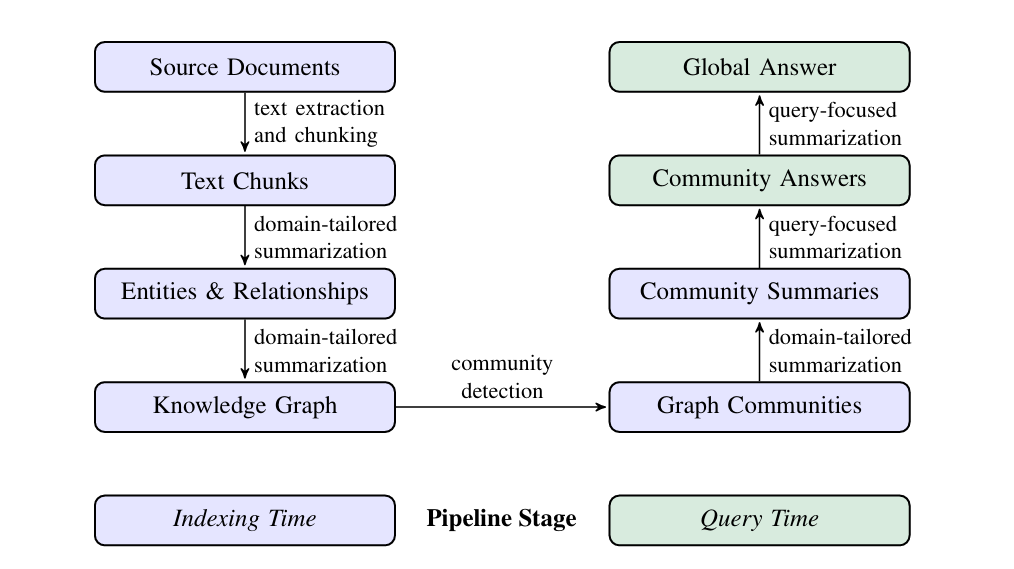
\includegraphics[width=0.8\textwidth]{figuri/graph.png}
  \caption{Arhitectura GraphRAG \cite{edge2024local}}
  \label{fig:graph}
\end{figure}

Figura~\ref{fig:graph} prezintă arhitectura generală a unui pipeline GraphRAG, organizat în două etape principale: etapa de indexare și etapa de interogare. În etapa de indexare, documentele sunt împărțite în fragmente, iar din aceste fragmente sunt extrase entități și relații. Informațiile obținute sunt organizate într-un graf de cunoștințe, în care nodurile reprezintă entități, iar muchiile descriu relațiile dintre acestea.

Pe baza grafului rezultat, sunt identificate comunități de noduri apropiate, care grupează concepte interconectate. Pentru aceste comunități sunt generate rezumate, astfel încât sistemul să dispună de o reprezentare sintetică a informației existente în graf. Această etapă este realizată înainte de interogarea efectivă, ca parte a procesului de indexare \cite{edge2024local}.

În etapa de interogare, rezumatele comunităților sunt utilizate pentru a genera răspunsuri parțiale relevante pentru întrebarea utilizatorului. Aceste răspunsuri parțiale sunt apoi combinate într-un răspuns global, printr-un proces de sumarizare orientat către interogare. Astfel, GraphRAG permite valorificarea structurii globale a corpusului, nu doar recuperarea locală a unor fragmente individuale \cite{edge2024local}.

Comparativ cu o abordare RAG bazată doar pe fragmente de text, utilizarea unui graf de cunoștințe poate oferi un context mai structurat și poate evidenția relații între concepte care nu sunt întotdeauna capturate prin similaritate vectorială. În cadrul proiectului, această idee este relevantă deoarece domeniul medical conține numeroase relații între simptome, afecțiuni, investigații și tratamente, iar reprezentarea acestor relații poate susține construirea unor răspunsuri mai bine contextualizate.


\subsection{Kuzu -- baza de date grafică}

Kuzu este o bază de date grafică de tip embedded, construită pentru viteză și scalabilitate în interogarea grafurilor \cite{kuzu_doc}. Spre deosebire de soluțiile de tip client-server, o bază de date embedded rulează în același proces cu aplicația care o utilizează, fără a necesita configurarea unui server separat. Această caracteristică simplifică integrarea în aplicații Python și este potrivită pentru proiecte în care prelucrarea grafului trebuie să fie strâns legată de logica aplicației.

Kuzu implementează modelul de date \textit{Property Graph} și oferă suport pentru limbajul de interogare Cypher \cite{kuzu_doc,kuzu_cidr}. În acest model, informația este reprezentată prin noduri și muchii, iar atât nodurile, cât și muchiile pot avea proprietăți asociate. Această structură este potrivită pentru reprezentarea relațiilor dintre concepte, deoarece permite modelarea explicită a legăturilor dintre entități și interogarea lor prin parcurgerea conexiunilor din graf.


\begin{figure}[H]
  \centering
  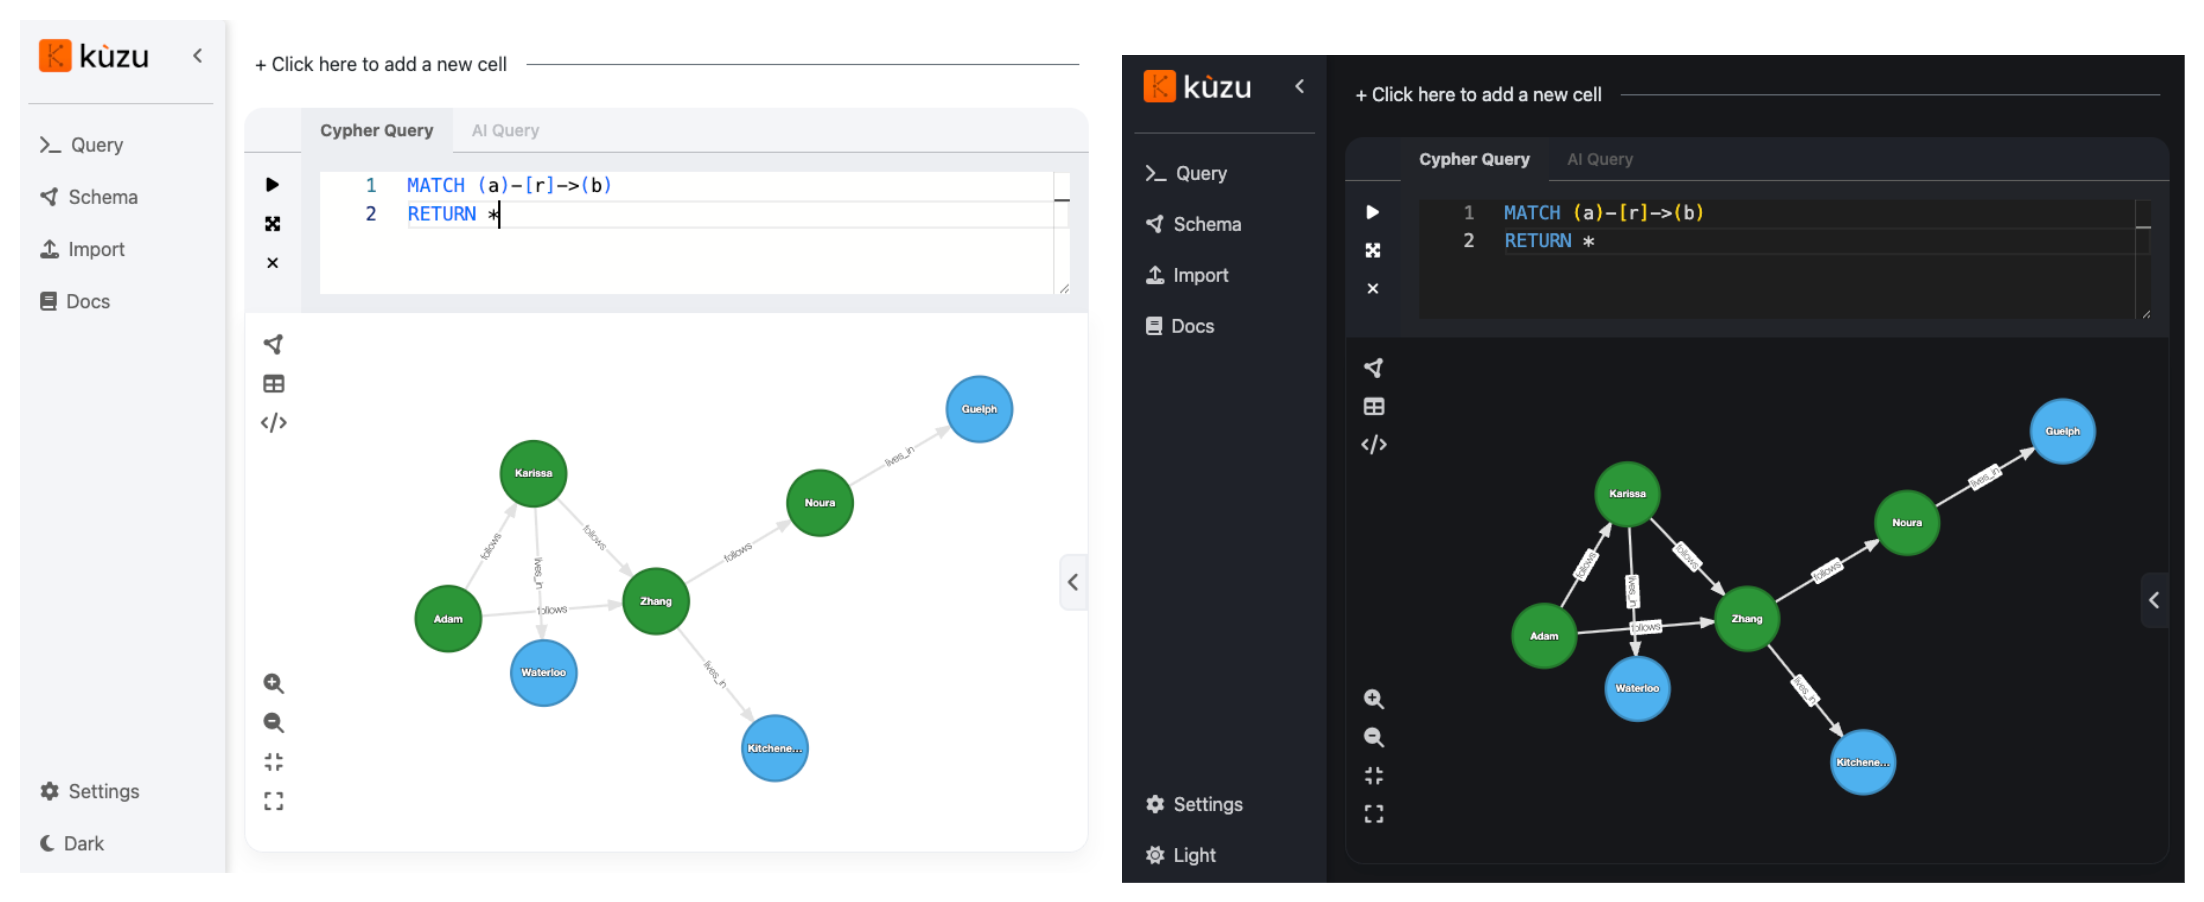
\includegraphics[width=0.9\textwidth]{figuri/explorer-graph-view.png}
  \caption{Interfața Kuzu Explorer \cite{kuzu_gdotv}}
  \label{fig:kuzu-explorer}
\end{figure}


În contextul unui sistem RAG extins cu o componentă grafică, Kuzu poate fi utilizat pentru stocarea și interogarea unui graf de cunoștințe extras din documentele sursă. Entitățile identificate în text pot fi reprezentate ca noduri, iar relațiile dintre acestea pot fi reprezentate ca muchii. Prin interogări asupra grafului, sistemul poate recupera nu doar fragmente similare textual, ci și informații legate prin relații explicite între concepte.

Construirea unui astfel de graf presupune identificarea entităților și a relațiilor din textul sursă. În procesarea limbajului natural, identificarea entităților este cunoscută sub denumirea de \textit{Named Entity Recognition}, iar identificarea legăturilor dintre acestea este asociată cu etapa de \textit{Relation Extraction}. Într-un domeniu medical, entitățile pot corespunde unor simptome, afecțiuni, investigații sau tratamente, iar relațiile pot exprima asocieri clinice, cauzale, terapeutice sau diagnostice.

În cadrul proiectului realizat, utilizarea Kuzu are rolul de a susține componenta de graf de cunoștințe. Aceasta completează regăsirea vectorială printr-o reprezentare structurată a relațiilor dintre concepte. Astfel, Qdrant este utilizat pentru căutarea semantică pe fragmente de text, în timp ce Kuzu poate fi utilizat pentru interogări relaționale asupra entităților și conexiunilor extrase din documente.

\section{Procesarea datelor și utilitare}

\subsection{Extracția textului din documente PDF cu PyMuPDF}

Documentele medicale utilizate ca sursă de cunoștințe sunt disponibile predominant în format PDF, un format opac din perspectiva prelucrării automate a textului. Extracția fidelă a conținutului textual reprezintă primul pas critic al pipeline-ului de ingestie, cu impact direct asupra calității informațiilor indexate.

PyMuPDF (denumit și \texttt{fitz}) este o bibliotecă Python de înaltă performanță pentru procesarea documentelor PDF, construită pe motorul MuPDF. Spre deosebire de alte soluții de extracție — precum \texttt{pdfminer} sau \texttt{pypdf} — PyMuPDF menține informații geometrice complete despre fiecare bloc de text: poziția, dimensiunea fontului și alinierea, permițând reconstruirea parțială a structurii logice a documentului pe baza proprietăților vizuale ale elementelor extrase.\cite{pymupdf_doc}

\subsection{Procesarea datelor tabelare cu modulul \texttt{csv}}

În implementarea curentă, datele tabelare sunt procesate cu modulul standard
\texttt{csv} din Python. Fișierul CSV este parcurs secvențial cu \texttt{csv.reader}, cu
validări explicite pe structură și pe câmpurile obligatorii înainte de
transformarea în obiecte tipizate \texttt{MedicalItem}. Această abordare menține
controlul strict asupra regulilor de validare și reduce complexitatea
operațională a pipeline-ului pentru seturile de date utilizate în proiect.


\subsection{Gestionarea configurației cu python-dotenv}

În aplicațiile software moderne, configurația sistemului este separată de codul sursă pentru a permite adaptarea mai ușoară la medii diferite de rulare, precum dezvoltare locală, testare sau producție. Configurația poate include adrese ale serviciilor externe, chei API, nume de baze de date, porturi de rețea, praguri de funcționare sau opțiuni prin care sunt activate anumite componente ale aplicației.

O practică frecvent utilizată este stocarea acestor valori în variabile de mediu. Variabilele de mediu permit aplicației să preia parametri externi fără ca aceștia să fie scriși direct în cod. Această abordare contribuie la creșterea flexibilității sistemului și la protejarea informațiilor sensibile, deoarece date precum cheile API, parolele sau tokenurile de acces nu trebuie incluse în fișierele sursă ale proiectului.

Biblioteca \texttt{python-dotenv} este utilizată în aplicațiile Python pentru citirea perechilor cheie--valoare dintr-un fișier \texttt{.env} și încărcarea acestora ca variabile de mediu \cite{python_dotenv_doc}. În mod uzual, aplicația apelează funcția \texttt{load\_dotenv()}, care citește valorile definite în fișierul \texttt{.env} și le adaugă în \texttt{os.environ}, astfel încât acestea pot fi accesate ulterior prin mecanismele standard ale limbajului Python, precum \texttt{os.getenv()} \cite{python_dotenv_doc}.

Fișierul \texttt{.env} conține variabile definite sub forma unor perechi de tip cheie--valoare, având o sintaxă asemănătoare cu cea utilizată în shell-urile de tip Bash \cite{python_dotenv_doc}. De exemplu, într-o aplicație care integrează servicii externe, acest fișier poate conține cheia API a furnizorului LLM, adresa unei baze de date vectoriale, numele modelului utilizat sau praguri pentru mecanismul de regăsire a contextului. Prin această metodă, modificarea configurației nu necesită schimbarea codului sursă, ci doar actualizarea valorilor din fișierul de configurare.

Un avantaj important al utilizării bibliotecii \texttt{python-dotenv} este susținerea principiilor aplicațiilor de tip \textit{12-factor}, unde configurația trebuie păstrată separat de codul aplicației \cite{python_dotenv_doc}. Această separare este utilă în special pentru aplicațiile care pot rula în medii diferite, deoarece aceeași bază de cod poate fi folosită cu setări diferite pentru dezvoltare, testare sau producție.

Din perspectiva securității, fișierul \texttt{.env} nu trebuie inclus în sistemul de versionare al proiectului dacă acesta conține informații sensibile. Documentația bibliotecii recomandă adăugarea fișierului \texttt{.env} în \texttt{.gitignore}, mai ales atunci când acesta conține secrete precum parole sau chei de acces \cite{python_dotenv_doc}. În practică, în repository se poate păstra un fișier exemplu, de tip \texttt{.env.example}, care descrie variabilele necesare aplicației, dar fără valori reale.

\section{Containerizare și rulare}

\subsection{Principiile containerizării cu Docker}

Docker este o platformă pentru containerizarea aplicațiilor software, 
oferind un mecanism de ambalare a aplicației împreună cu dependențele 
și configurațiile sale într-o imagine portabilă și reproductibilă 
\cite{docker_doc}. Containerele Docker folosesc mecanisme ale nucleului Linux, precum namespace-urile și cgroup-urile, pentru a oferi izolare la nivel de proces și control asupra resurselor. Namespace-urile izolează resursele sistemului — sistem de fișiere, rețea, procese — încât fiecare container are propria 
vedere asupra acestora, iar cgroup-urile limitează și monitorizează utilizarea 
resurselor precum CPU și memorie \cite{docker_doc}. În practică, această abordare asigură un mediu de execuție mult mai consistent între dezvoltare, testare și producție și reduce problemele clasice de incompatibilitate a dependențelor, fără a implica însă izolarea completă specifică unei mașini virtuale.

Imaginea Docker a proiectului este definită printr-un fișier 
\texttt{Dockerfile} single-stage, care instalează dependențele și 
uneltele necesare în aceeași imagine de execuție. Această abordare 
simplifică procesul de compilare și este adecvată mediului de dezvoltare, 
unde prioritatea este reproductibilitatea mediului de execuție, nu 
optimizarea dimensiunii imaginii finale \cite{docker_doc}.

\subsection{Orchestrarea serviciilor cu Docker Compose}

Aplicația este compusă din mai multe servicii independente care trebuie să funcționeze coordonat pentru a oferi funcționalitate completă. Docker Compose permite definirea și gestionarea acestor servicii printr-un fișier YAML unic, simplificând semnificativ procesul de pornire, oprire și configurare a întregii stive aplicative \cite{docker_compose_doc}.

Topologia Docker Compose a proiectului include următoarele servicii:
\begin{itemize}
  \item \texttt{app} — serviciu CLI pentru rularea aplicației prin entrypoint-ul principal run.py,
  incluzând chat interactiv, ingestie și evaluare;
  \item \texttt{api} — serviciu Flask care expune funcționalitățile chatbotului prin interfață REST
  și endpoint-uri compatibile cu clienți externi.;
  \item \texttt{qdrant} — baza de date vectorială, rulată ca serviciu 
  persistent cu stocare montată pe sistemul gazdă;
  \item \texttt{openwebui} — front-end-ul grafic pentru interacțiunea 
  conversațională;
  \item \texttt{kuzu-explorer} — interfața grafică pentru Kuzu;
  \item \texttt{ollama} — serviciu opțional pentru inferența locală, 
  activat prin profilul \texttt{local-llm}.
\end{itemize}

\subsection{Reproductibilitatea mediului de execuție}

Containerizarea garantează reproductibilitatea completă a mediului de execuție: orice utilizator care pornește stiva Docker Compose pornind de la aceeași configurație va obține un mediu funcțional identic cu cel utilizat în dezvoltare și testare. Această proprietate este esențială în contextul cercetării și evaluării academice, unde reproductibilitatea rezultatelor reprezintă un criteriu fundamental de validitate științifică \cite{reproducibility2018}.

Fișierul \texttt{.env.example} inclus în repository documentează  toate variabilele de mediu necesare pentru configurarea sistemului, cu valori implicite sigure și comentarii explicative. Acest fișier template simplifică procesul de configurare inițială și reduce bariera de intrare pentru noi utilizatori sau evaluatori ai sistemului.

\section{Calitatea codului și testare}

\subsection{Instrumente de formatare și analiză statică}

Menținerea unui standard uniform al stilului de cod este importantă în proiectele cu arhitectură modulară, deoarece facilitează citirea, revizuirea și extinderea codului pe durata întregului ciclu de viață al proiectului. Proiectul utilizează Black ca formator automat de cod Python \cite{black_doc}. Black aplică un stil de formatare opinionat și neambiguu, eliminând necesitatea deciziilor manuale de formatare și asigurând uniformitatea vizuală a întregii baze de cod.

Ruff este un linter Python de înaltă performanță, implementat în Rust \cite{ruff_doc}, care verifică respectarea unui set extins de reguli de calitate a codului: detecția variabilelor neutilizate, a importurilor redundante sau incorect ordonate, a anti-pattern-urilor comune și a potențialelor erori logice. Spre deosebire de soluțiile tradiționale de analiză statică, Ruff oferă o performanță de zeci de ori mai rapidă \cite{ruff_doc}, permițând integrarea sa ca pas de verificare în pipeline-ul de CI/CD fără impact semnificativ asupra timpului total de build.

\subsection{Cadrul de testare automată}

Proiectul include o suită extinsă de teste automate, organizată pe două niveluri de abstractizare. Testele unitare verifică comportamentul corect al componentelor individuale în izolare, prin furnizarea dependențelor simulate care elimină efectele colaterale ale apelurilor externe. Testele de integrare verifică comportamentul fluxurilor complete de execuție, asigurând că interacțiunile dintre componente se desfășoară conform așteptărilor.

Testele sunt implementate în principal cu framework-ul standard \texttt{unittest}, iar execuția este realizată prin comenzi de tip \texttt{python -m unittest}. Suita de teste acoperă componentele critice ale sistemului. Modulul de protecție (\textit{guardrails}) este verificat pentru detectarea interogărilor periculoase, a mesajelor de urgență și a conținutului din afara domeniului medical. Modulul de orchestrare este testat pentru construcția promptului și pentru logica de reluare în caz de evaluare eșuată. Modulele de regasire a informației sunt verificate pentru corectitudinea extracției, segmentării și indexării documentelor.

\subsection{Monitorizarea acoperirii testelor}

Acoperirea testelor (\textit{test coverage}) este monitorizată prin instrumentul \texttt{coverage.py} \cite{coveragepy_doc}, care măsoară procentul de linii de cod executate în cursul rulării complete a suitei de teste. Deși o acoperire ridicată nu garantează în sine absența defectelor, ea oferă un indicator obiectiv al gradului în care comportamentul sistemului este validat și documentat prin scenarii explicite.

Rapoartele de acoperire sunt generate periodic și urmărite ca metrică de calitate pe parcursul dezvoltării proiectului. Componentele cu acoperire redusă sunt identificate și prioritizate pentru completarea suitei de teste în iterațiile ulterioare, menținând un nivel ridicat de încredere în stabilitatea funcțională a sistemului pe măsura extinderii sale.

\chapter{Arhitectura proiectului}

\section{Arhitectura de ansamblu}
\label{sec:ansamblu}

Sistemul implementat este organizat ca o arhitectură modulară de tip agentic, în care fiecare componentă are un rol clar și poate fi testată, înlocuită sau extinsă independent. Pentru a respecta principiul separării responsabilităților (\textit{separation of concerns}), proiectul este împărțit în module specializate, fiecare cu o funcție bine definită:
\begin{itemize}
    \item \texttt{agent} coordonează fluxul principal al cererii: aplicarea regulilor de protecție, rularea motorului de raționament, evaluarea răspunsului și gestionarea reluărilor (\textit{retry});
    \item \texttt{rag} se ocupă de pregătirea și regăsirea contextului: segmentează documentele, generează embedding-uri și interogheaza baza vectorială pentru fragmente relevante;
    \item \texttt{knowledge} gestionează componenta de graf de cunoștințe, inclusiv extracția entităților medicale și reprezentarea relațiilor dintre acestea;
    \item \texttt{api} expune funcționalitatea sistemului prin endpoint-uri REST, astfel încât aplicația să poată fi folosită din interfețe externe;
    \item \texttt{config} centralizează parametrii de configurare și șabloanele de prompt, pentru a menține comportamentul sistemului consecvent și ușor de ajustat.
\end{itemize}
Contractele de date dintre module sunt definite explicit în pachetul \texttt{models}, prin clase \texttt{dataclass} tipizate, completate de validări în punctele critice de intrare, pentru a menține consistența tipurilor pe întregul flux de execuție.

Interdependențele dintre module sunt gestionate exclusiv prin furnizarea dependențelor: fiecare componentă primește funcțiile de care are nevoie ca parametri la inițializare, fără a instanția direct dependențele sale. Această decizie de proiectare are două consecințe practice: facilitarea testării — orice componentă poate fi testată izolat prin substituirea dependențelor cu implementări simulate — și extensibilitatea — un nou furnizor LLM sau o nouă strategie de regăsire pot fi integrate fără modificări în logica de orchestrare.

Fluxul de procesare al unei interogări urmează o succesiune secvențială de etape, proiectată pentru a reduce riscul de răspunsuri incorecte în context medical. Figura~\ref{fig:pipeline} ilustrează această succesiune.

\begin{figure}[H]
\centering
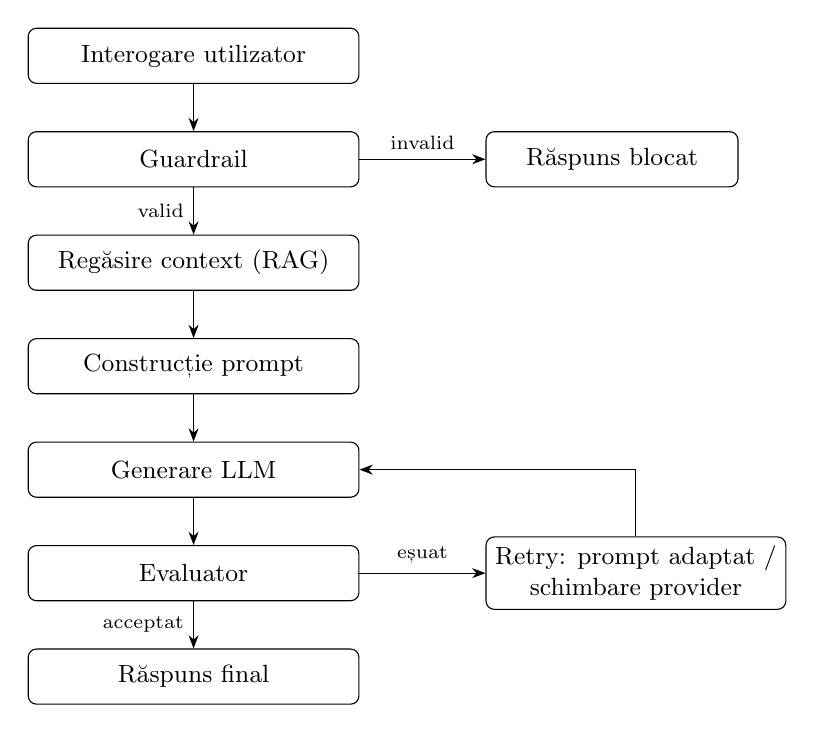
\begin{tikzpicture}[
  box/.style={draw, rounded corners=3pt, minimum width=4.2cm, minimum height=0.7cm, align=center, font=\small},
  sidebox/.style={draw, rounded corners=3pt, minimum width=3.2cm, minimum height=0.7cm, align=center, font=\small},
  >=Stealth, node distance=0.6cm
]
\node[box] (q)   {Interogare utilizator};
\node[box, below=of q]   (g)   {Guardrail};
\node[sidebox, right=1.6cm of g] (bl)  {\small Răspuns blocat};
\node[box, below=of g]   (rag) {Regăsire context (RAG)};
\node[box, below=of rag] (pr)  {Construcție prompt};
\node[box, below=of pr]  (llm) {Generare LLM};
\node[box, below=of llm] (ev)  {Evaluator};
\node[sidebox, right=1.6cm of ev] (rt)  {\small Retry: prompt adaptat /\\ schimbare provider};
\node[box, below=of ev]  (out) {Răspuns final};

\draw[->] (q)   -- (g);
\draw[->] (g)   -- node[left]{\scriptsize valid}   (rag);
\draw[->] (g)   -- node[above]{\scriptsize invalid} (bl);
\draw[->] (rag) -- (pr);
\draw[->] (pr)  -- (llm);
\draw[->] (llm) -- (ev);
\draw[->] (ev)  -- node[left]{\scriptsize acceptat} (out);
\draw[->] (ev)  -- node[above]{\scriptsize eșuat}   (rt);
\draw[->] (rt.north) |- (llm.east);
\end{tikzpicture}
\caption{Fluxul de procesare al unei interogări în sistemul chatbot medical}
\label{fig:pipeline}
\end{figure}

În implementarea proiectului, etapa de regăsire include și o verificare a pragului minim de relevanță, configurat prin variabila \texttt{RETRIEVAL\_MIN\_SCORE}. Valoarea implicită este \texttt{0.2}. Dacă nu sunt recuperate fragmente relevante sau dacă scorul maxim al fragmentelor recuperate este sub acest prag, motorul de raționament returnează direct un mesaj de încredere scăzută, fără a mai apela modelul LLM.

\begin{enumerate}
    \item aplicarea mecanismelor de protecție (\textit{guardrails}) asupra întrebării utilizatorului;
    \item delegarea către modulul de \textit{reasoning}, care decide dacă este necesară recuperarea de context din baza vectorială (RAG);
    \item extragerea fragmentelor relevante atunci când interogarea necesită cunoștințe externe;
    \item construirea promptului final prin combinarea regulilor din fișierul \texttt{llm.txt}, a contextului recuperat și a întrebării utilizatorului;
    \item trimiterea promptului către LLM Hub și generarea răspunsului;
    \item evaluarea răspunsului cu un evaluator dedicat;
    \item reluarea procesului, în modulul de \textit{reasoning}, cu prompt ajustat sau cu schimbarea furnizorului LLM, dacă evaluarea nu este satisfăcătoare;
    \item returnarea către utilizator doar a răspunsului validat.
\end{enumerate}


\section{Orchestratorul}

Orchestratorul reprezintă punctul central de coordonare al sistemului, responsabil cu execuția completă a ciclului de viață al unei cereri: validare prin guardrail, regăsire de context, generare de răspuns, evaluare și, dacă este necesar, reluare. Implementat în clasa \texttt{Orchestrator} din \texttt{agent/orchestrator/orchestrator.py}, acesta primește o cerere de interogare și returnează un răspuns complet, adnotat cu rezultatele tuturor etapelor intermediare.

\begin{figure}[H]
\centering
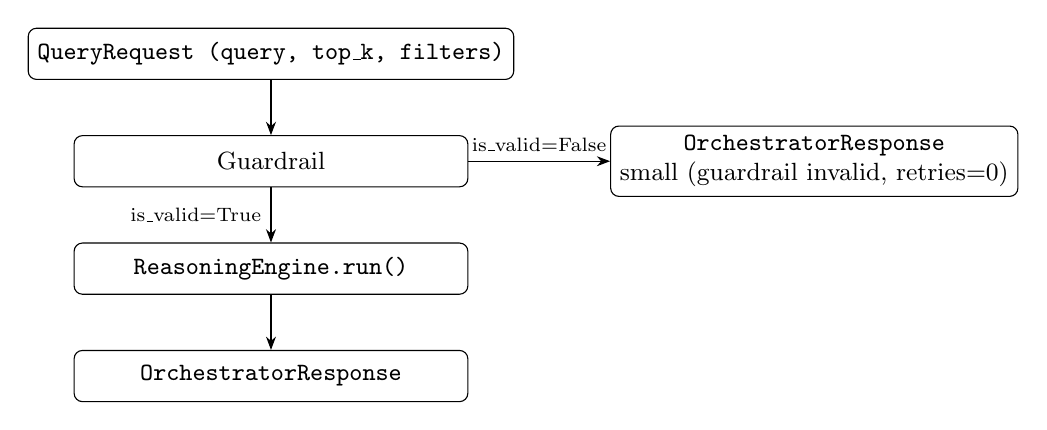
\begin{tikzpicture}[
  box/.style={draw, rounded corners=3pt, minimum width=5cm, minimum height=0.65cm, align=center, font=\small},
  sbox/.style={draw, rounded corners=3pt, minimum width=3.8cm, minimum height=0.65cm, align=center, font=\small},
  >=Stealth, node distance=0.7cm
]
\node[box] (req)  {\texttt{QueryRequest (query, top\_k, filters)}};
\node[box, below=of req]  (grd)  {Guardrail};
\node[sbox, right=1.8cm of grd] (blk)  {\small \texttt{OrchestratorResponse}\\small (guardrail invalid, retries=0)};
\node[box, below=of grd]  (re)   {\texttt{ReasoningEngine.run()}};
\node[box, below=of re]   (resp) {\texttt{OrchestratorResponse}};

\draw[->] (req) -- (grd);
\draw[->] (grd) -- node[left]{\scriptsize is\_valid=True}  (re);
\draw[->] (grd) -- node[above]{\scriptsize is\_valid=False} (blk);
\draw[->] (re)  -- (resp);
\end{tikzpicture}
\caption{Fluxul de execuție al \texttt{Orchestrator.run()}}
\label{fig:orchestrator}
\end{figure}

\subsection{Structura și gestionarea de dependențe}

Orchestratorul utilizează un model de organizare a dependențelor prin intermediul 
clasei \texttt{OrchestratorDependencies}, care grupează toate funcțiile externe necesare: \texttt{guardrail} (implicit \texttt{apply\_guardrails}), \texttt{retrieve} (implicit \texttt{retrieve\_top\_similar}), \texttt{llm\_call} (implicit \texttt{llm\_ask\_request}) și \texttt{evaluator} (implicit \texttt{evaluate\_response}). Această arhitectură permite înlocuirea oricărei componente cu versiuni de test în timpul testării, fără a modifica logica de orchestrare. La inițializare, orchestratorul construiește intern un \texttt{ReasoningEngine} căruia îi transmite aceleași dependențe, delegând acestuia toată logica de generare și evaluare.

\subsection{Fluxul de execuție}

Metoda \texttt{run} primește un obiect \texttt{QueryRequest} cu câmpurile \texttt{query}, \texttt{top\_k} (implicit 3), \texttt{language} (implicit \texttt{"ro"}) și \texttt{filters} opționale. Execuția urmează două etape secvențiale:

\begin{enumerate}
    \item \textbf{Validarea prin guardrail}: interogarea este transmisă funcției de guardrail. Dacă rezultatul are \texttt{is\_valid = False}, orchestratorul returnează imediat un \texttt{OrchestratorResponse} cu mesajul de respingere al guardrailului, fără a apela motorul de raționament. Numărul de reluări este 0, iar câmpurile \texttt{evaluator} și \texttt{retrieval} sunt \texttt{None}.
    \item \textbf{Reasoning}: dacă interogarea este validă, controlul este transferat la  \texttt{ReasoningEngine} printr-un \texttt{ReasoningInput} ce conține interogarea, \texttt{top\_k}, limba și filtrele. Rezultatul \texttt{ReasoningOutput} este prelucrat direct în câmpurile \texttt{OrchestratorResponse}: răspunsul final, furnizorul și modelul utilizat, numărul de reluări, rezultatul evaluatorului, rezultatul regăsirii și liniile de context.
\end{enumerate}

Logica completă de regăsire a contextului, construcție a promptului, generare, evaluare și reluare este implementată în \texttt{ReasoningEngine} și este descrisă în detaliu în secțiunea~\ref{sec:reasoning}. Orchestratorul nu reproduce această logică — el o invocă printr-un apel unic la metoda \texttt{run}, primind înapoi un \texttt{ReasoningOutput} complet care include răspunsul, proveniența și istoricul procesului de generare.

\subsection{Structura răspunsului final}

Orchestratorul returnează un obiect \texttt{OrchestratorResponse} cu câmpurile: \texttt{response} (textul răspunsului sau \texttt{None}), \texttt{provider} și \texttt{model} (furnizorul și modelul utilizat la ultima generare), \texttt{retries} (numărul de reluări efectuate), \texttt{guardrail} (\texttt{GuardrailResult} cu detaliile validării), \texttt{evaluator} (\texttt{EvaluatorResult} sau \texttt{None} în caz de respingere de guardrail), \texttt{retrieval} (\texttt{RetrievalResult} sau \texttt{None}) și \texttt{context\_lines} (lista liniilor de context utilizate). Structura serializabilă a acestui obiect permite API-ului să returneze clientului informații complete, asigurând transparența întregului proces de generare.


\section{Modulul de raționament (Reasoning)}
\label{sec:reasoning}

Modulul de raționament, implementat în clasa \texttt{ReasoningEngine} din \texttt{agent/reasoning/engine.py}, concentrează întreaga logică de decizie privind generarea răspunsului: recuperarea și validarea contextului RAG, construcția promptului, evaluarea calității și strategia de reluare. Orchestratorul îi deleagă controlul complet după ce guardrail-ul validează interogarea, iar \texttt{ReasoningEngine} returnează un răspuns final validat sau un mesaj de încredere scăzută.

\subsection{Preprocesarea interogării și validarea contextului RAG}

Prima etapă a motorului de raționament constă în evaluarea directă a interogării utilizatorului pentru regăsire contextuală. Interogarea este transmisă modulului RAG fără transformări lingvistice intermediare, iar motorul verifică dacă există fragmente relevante și dacă scorul maxim depășește pragul minim configurat (\texttt{retrieval\_min\_score}). Dacă nu, răspunsul este un mesaj de încredere scăzută returnat direct, fără a mai apela modelul LLM — evitând astfel generarea de răspunsuri nefondate în absența unui context relevant.

\subsection{Construcția promptului și generarea răspunsului}

Dacă regăsirea produce context relevant, fragmentele sunt asamblate într-un bloc de context structurat. Promptul final combină sistemul de instrucțiuni din \texttt{llm.txt}, blocul de context și interogarea originală a utilizatorului.

Generarea se desfășoară într-o buclă cu un număr maxim de încercări configurat. La fiecare iterație, motorul selectează furnizorul LLM activ, trimite cererea și evaluează răspunsul primit. Dacă evaluatorul semnalează un răspuns valid sau nu recomandă reluarea, bucla se oprește. Altfel, se aplică una din două strategii de reluare, în funcție de tipul de eșec detectat de evaluator:

\begin{itemize}
    \item \textbf{Prompt ajustat} (\texttt{adjust\_prompt}) — mesajul utilizatorului este completat cu instrucțiuni corective derivate din motivele de eșec raportate de evaluator, ghidând modelul spre un răspuns mai precis în aceeași încercare;
    \item \textbf{Schimbarea furnizorului} (\texttt{switch\_llm}) — dacă modelul curent are dificultăți cu tipul de interogare, motorul comută pe următorul furnizor din ierarhia de fallback configurată, menținând același prompt.
\end{itemize}

\subsection{Rutarea multi-provider}

Selecția furnizorului pentru fiecare încercare este gestionată de metoda \texttt{\_select\_provider}. La prima încercare se folosește întotdeauna furnizorul primar configurat prin variabile de mediu. Pentru încercările ulterioare cu strategia \texttt{switch\_llm}, motorul parcurge în ordine lista \texttt{provider\_fallback\_order} din configurația evaluatorului. Dacă lista este epuizată, revine la furnizorul primar. Clienții concreți pentru OpenAI, Anthropic și modelele locale (Gemma, Qwen prin Ollama) sunt implementați în \texttt{agent/reasoning/providers/} și expuși printr-o interfață unificată în \texttt{llm/llm\_router.py}.

\subsection{Finalizarea răspunsului}

După ieșirea din buclă, răspunsul final este completat cu blocul fragmentelor recuperate și, în modul hibrid de regăsire, cu un bloc de citări structurate ce include sursa și pagina fiecărui fragment utilizat. Motorul returnează un obiect \texttt{ReasoningOutput} care include răspunsul, furnizorul și modelul folosit, numărul de reluări, rezultatul evaluatorului și rezultatul regăsirii — oferind orchestratorului transparență completă asupra procesului de generare.




\section{Modulul de protecție (Guardrails)}

Modulul de protecție reprezintă prima componentă prin care trece orice interogare a utilizatorului și are rolul de a determina dacă aceasta poate fi procesată în continuare de sistem. Decizia se bazează pe o strategie în două niveluri: o verificare deterministă bazată pe șabloane de cuvinte-cheie, urmată, la nevoie, de o clasificare semantică realizată de un model LLM.

\subsection{Motivația și rolul modulului}

Într-un sistem de tip chatbot medical, riscurile asociate unui răspuns neadecvat sunt semnificativ mai ridicate decât în aplicații de uz general. Un utilizator poate descrie o urgență medicală reală, poate solicita doze precise de medicamente sau poate formula întrebări cu intenții vătămătoare. Fără un mecanism explicit de filtrare, sistemul ar putea genera răspunsuri care, deși corecte din perspectivă lingvistică, pot constitui sfaturi periculoase sau pot întârzia accesul la îngrijire medicală de urgență.

Modulul de protecție adresează aceste riscuri prin clasificarea fiecărei interogări într-una din categoriile definite și prin blocarea sau redirecționarea celor care nu pot fi procesate în siguranță de sistemul de generare.

\begin{figure}[H]
\centering
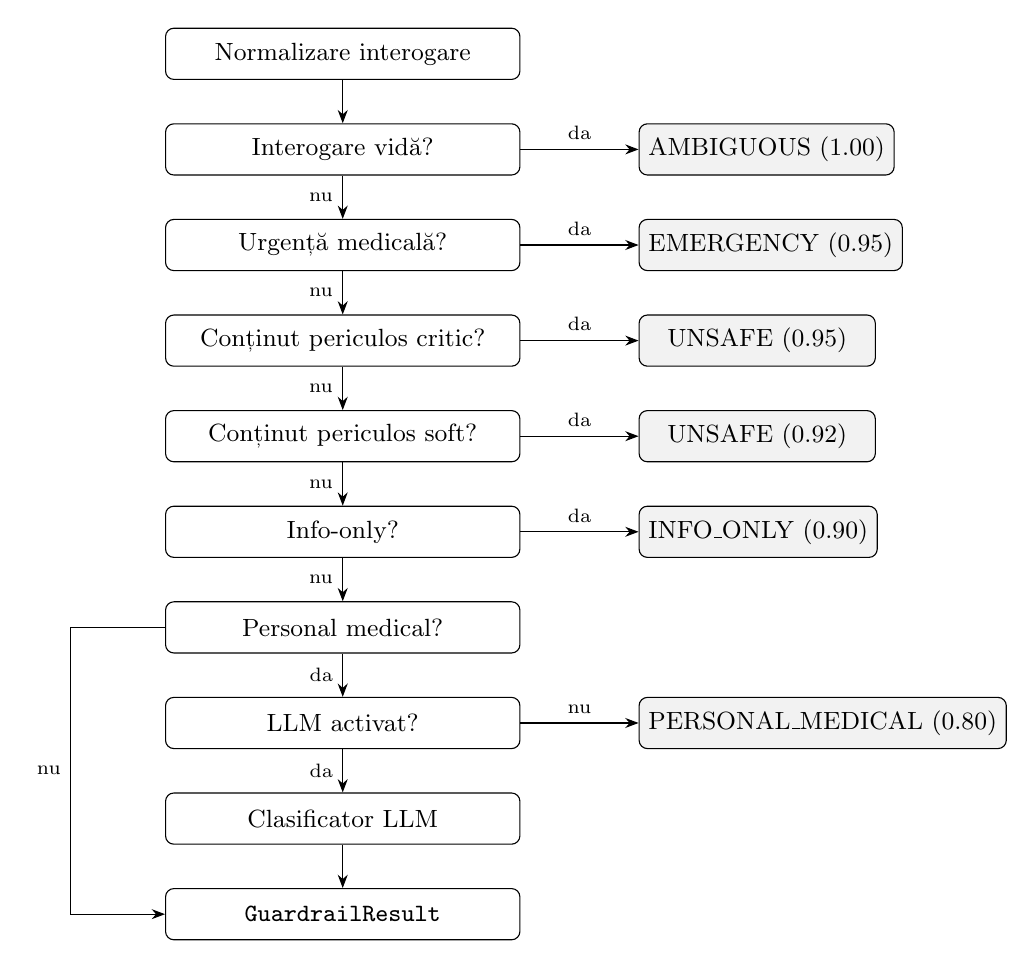
\begin{tikzpicture}[
  box/.style={draw, rounded corners=3pt, minimum width=4.5cm, minimum height=0.65cm, align=center, font=\small},
  res/.style={draw, rounded corners=3pt, minimum width=3cm, minimum height=0.65cm, align=center, font=\small, fill=gray!10},
  >=Stealth, node distance=0.55cm
]
\node[box] (norm) {Normalizare interogare};
\node[box, below=of norm] (v1) {Interogare vidă?};
\node[res, right=1.5cm of v1] (r1) {AMBIGUOUS (1.00)};
\node[box, below=of v1] (v2) {Urgență medicală?};
\node[res, right=1.5cm of v2] (r2) {EMERGENCY (0.95)};
\node[box, below=of v2] (v3) {Conținut periculos critic?};
\node[res, right=1.5cm of v3] (r3) {UNSAFE (0.95)};
\node[box, below=of v3] (v4) {Conținut periculos soft?};
\node[res, right=1.5cm of v4] (r4) {UNSAFE (0.92)};
\node[box, below=of v4] (v5) {Info-only?};
\node[res, right=1.5cm of v5] (r5) {INFO\_ONLY (0.90)};
\node[box, below=of v5] (v6) {Personal medical?};
\node[box, below=of v6] (llmon) {LLM activat?};
\node[res, right=1.5cm of llmon] (r6) {PERSONAL\_MEDICAL (0.80)};
\node[box, below=of llmon] (llm) {Clasificator LLM};
\node[box, below=of llm] (gr) {\texttt{GuardrailResult}};

% Flux principal vertical
\draw[->] (norm)  -- (v1);
\draw[->] (v1)    -- node[left]{\scriptsize nu} (v2);
\draw[->] (v2)    -- node[left]{\scriptsize nu} (v3);
\draw[->] (v3)    -- node[left]{\scriptsize nu} (v4);
\draw[->] (v4)    -- node[left]{\scriptsize nu} (v5);
\draw[->] (v5)    -- node[left]{\scriptsize nu} (v6);
\draw[->] (v6)    -- node[left]{\scriptsize da} (llmon);
\draw[->] (llmon) -- node[left]{\scriptsize da} (llm);
\draw[->] (llm)   -- (gr);

% Rezultate la dreapta
\draw[->] (v1)    -- node[above]{\scriptsize da} (r1);
\draw[->] (v2)    -- node[above]{\scriptsize da} (r2);
\draw[->] (v3)    -- node[above]{\scriptsize da} (r3);
\draw[->] (v4)    -- node[above]{\scriptsize da} (r4);
\draw[->] (v5)    -- node[above]{\scriptsize da} (r5);
% LLM dezactivat → PERSONAL_MEDICAL cu scor mic
\draw[->] (llmon) -- node[above]{\scriptsize nu} (r6);

% "nu" de la Personal medical → GuardrailResult pe stânga
\draw[->] (v6.west)
  -- ++(-1.2, 0)
  |- node[pos=0.25, left]{\scriptsize nu} (gr.west);

\end{tikzpicture}
\caption{Strategia de clasificare a modulului Guardrail}
\label{fig:guardrail}
\end{figure}

Clasificatorul LLM este utilizat doar pentru interogări personale medicale și numai dacă opțiunea \texttt{GUARDRAIL\_LLM\_ENABLED} este activă. În caz contrar, interogarea este acceptată direct ca \texttt{PERSONAL\_MEDICAL}. Dacă este apelat, clasificatorul poate confirma categoria personal medicală sau poate respinge interogarea ca urgență, conținut nesigur ori întrebare ambiguă.


\subsection{Categoriile de clasificare}

Sistemul definește șase categorii de clasificare, fiecare asociată cu o politică de răspuns distinctă:

\begin{itemize}
    \item \textbf{EMERGENCY} — interogarea conține indicatori ai unei urgențe medicale imediate (ex. durere în piept, dificultăți de respirație, accident vascular cerebral). Sistemul blochează procesarea ulterioară și returnează un mesaj care îndeamnă utilizatorul să contacteze serviciile de urgență (numărul 112).
    \item \textbf{UNSAFE} — interogarea conține conținut explicit dăunător. Sunt definite două sub-variante: critica, care acoperă intenții de autoagresiune, violență sau sinteză de substanțe interzise, și soft, care vizează solicitări de doze exacte, prescripții sau scheme personalizate de tratament fără consultarea unui medic. Ambele variante blochează răspunsul, dar furnizează mesaje diferite adaptate situației.
    \item \textbf{AMBIGUOUS} — interogarea este ambiguă sau nu poate fi clasificată cu suficientă certitudine. Sistemul returnează un mesaj de redirecționare către un medic.
    \item \textbf{INFO\_ONLY} — interogarea are caracter informațional pur (definiții, simptome generale, cauze, prevenție) și nu conține indicatori personali sau de urgență. Este considerată validă și este transmisă mai departe în pipeline.
    \item \textbf{PERSONAL\_MEDICAL} — interogarea conține markeri la persoana întâi (ex. „am durere", „mă simt"), sugerând o situație personală, nu educațională. Este considerată validă, dar semnalată orchestratorului pentru o tratare diferențiată.
    \item \textbf{SAFE} — interogarea nu a declanșat niciun șablon specific și este considerată sigură. Este transmisă mai departe în pipeline.
\end{itemize}

Fiecărei categorii îi este asociat un scor de încredere care reflectă gradul de certitudine al deciziei. Politica de acordare a scorurilor este: 1,00 pentru respingerea interogărilor vide, 0,95 pentru potriviri deterministe cu risc ridicat (urgențe și conținut periculos critic), 0,92 pentru potriviri soft nesigure, 0,90 pentru clasificări deterministe inofensive, 0,80 pentru decizii luate pe baza LLM și 0,60 pentru situațiile în care LLM-ul nu este disponibil.

\subsection{Strategia deterministă de clasificare}

Prima fază a modulului utilizează potriviri de șabloane de cuvinte-cheie organizate ierarhic în grupuri tematice. Interogarea este normalizată înainte de aplicarea șabloanelor — prin conversia la litere mici și eliminarea diacriticelor — pentru a reduce variabilitatea lingvistică și a îmbunătăți rata de detecție.

Verificările se aplică în ordine strict ierarhică, ceea ce garantează că riscurile cu impact mai mare sunt evaluate primele:

\begin{enumerate}
    \item \textbf{Interogare vidă}: o interogare goală sau formată exclusiv din spații este respinsă imediat, cu un scor de încredere de 1,00.
    \item \textbf{Șabloane de urgență}: grupuri de expresii acoperind urgențe cardiovasculare, respiratorii, neurologice, traumatisme hemoragice și supradoze sau intoxicații. Dacă se detectează o potrivire și contextul nu este pur educațional, interogarea este clasificată \textbf{EMERGENCY} cu scor 0,95.
    \item \textbf{Șabloane critice nesigure}: expresii cu intenții de autoagresiune, violență sau sinteză de substanțe periculoase. La detectare, interogarea este clasificată \textbf{UNSAFE} cu scor 0,95.
    \item \textbf{Șabloane soft nesigure}: solicitări de doze exacte, prescripții sau scheme de tratament personalizate. La detectare, interogarea este clasificată \textbf{UNSAFE} cu scor 0,92.
    \item \textbf{Markeri informativi și personali}: expresii cu caracter educațional sau cu referire la persoana întâi, pentru clasificarea în \textbf{INFO\_ONLY} sau \textbf{PERSONAL\_MEDICAL} cu scor 0,90.
\end{enumerate}

Un mecanism special previne false pozitive pentru categoria de urgență: o interogare care conține expresii de urgență, dar care prezintă și un cadru educațional evident (ex. „ce simptome are un infarct?"), fără markeri personali sau de urgență imediată, nu este clasificată ca EMERGENCY. Această detectare a contextului educațional se realizează prin verificarea simultană a prezenței unor semnale educaționale și a absenței markerilor la persoana întâi și a indicatorilor de urgență actuală.

\subsection{Clasificarea asistată de LLM}

Abordarea hibridă — deterministă mai întâi, LLM ulterior — este justificată de necesitatea echilibrului între viteză și acuratețe semantică. Verificările pe bază de șabloane sunt instantanee și acoperă cazurile cu risc ridicat, bine definite lexical (urgențe, doze, automutilare). LLM-ul este invocat doar pentru interogările care nu au primit o clasificare certă, ceea ce limitează latența suplimentară la cazurile cu adevărat ambigue și reduce costul de inferență.

Interogările care nu primesc o clasificare deterministă certă — în special cele cu caracter personal sau ambiguu — sunt trimise spre clasificare semantică unui model LLM. Modelul primește un prompt de sistem cu instrucțiuni stricte și trebuie să returneze exact una dintre etichetele predefinite: \texttt{EMERGENCY}, \texttt{UNSAFE}, \texttt{SAFE} sau \texttt{AMBIGUOUS}.

Temperatura LLM este setată la zero pentru a elimina variabilitatea și a asigura reproductibilitatea deciziilor. Dacă răspunsul modelului nu corespunde exact uneia dintre etichete, se aplică o potrivire fuzzy: dacă denumirea unei categorii cu risc este conținută ca subșir în răspunsul brut, aceasta este selectată. Dacă nicio potrivire nu reușește, clasificatorul revine implicit la \texttt{SAFE}, evitând blocarea nejustificată a interogărilor benigne.

În cazul în care modelul LLM nu este disponibil (eroare de rețea, depășirea timpului de răspuns etc.), modulul revine la un rezultat \textbf{SAFE} cu scor de încredere 0,60, asigurând disponibilitatea serviciului chiar și în absența clasificatorului semantic.

\subsection{Structura rezultatului}

Indiferent de calea de clasificare urmată, modulul returnează un obiect \texttt{GuardrailResult} care include: categoria de clasificare, codul motivului deciziei, scorul de încredere, indicatorul de validitate al interogării, cuvintele-cheie care au declanșat decizia și un indicator boolean care arată dacă a fost utilizat LLM-ul. Această structură permite orchestratorului să ia decizii informate și oferă transparență completă pentru validarea comportamentului sistemului.


Fiecare decizie este înregistrată în jurnalul de evenimente al aplicației cu nivel \texttt{INFO} pentru deciziile sigure sau \texttt{WARNING} pentru deciziile de blocare, facilitând monitorizarea și depanarea în producție.

\section{Modulul RAG}

Modulul RAG are rolul de a furniza modelului LLM context factual relevant extras din baza de cunoștințe a sistemului. Acesta acoperă întregul pipeline de la ingestia documentelor până la regăsirea fragmentelor la momentul interogării.

\subsection{Pipeline-ul de extracție și preprocesare a documentelor}

O abordare naivă de extracție PDF — în care întregul document este procesat ca un singur bloc de text — s-a dovedit insuficientă în contextul documentelor medicale utilizate. Documentele de tip curs sau ghid clinic prezintă frecvent artefacte de extracție semnificative: text reordonat față de fluxul logic al paginii, coloane detectate incorect, antete și subsoluri intercalate în corp, formule sau tabele transformate în șiruri de caractere fără semnificație.

Pentru a rezolva aceste limitări, a fost proiectat un pipeline de extracție în trei etape. În \textbf{prima etapă}, PyMuPDF parcurge documentul pagină cu pagină, extragând independent conținutul textual al fiecărei pagini sub formă de bloc brut. Procesarea individuală a paginilor permite izolarea artefactelor la nivelul paginii de origine și simplifică etapele ulterioare de corecție.

În \textbf{a doua etapă}, textul brut al fiecărei pagini este transmis unui model LLM cu un prompt specializat. În implementarea proiectului, promptul cere explicit păstrarea conținutului factual, eliminarea elementelor parazite recurente — antete, subsoluri, numere de pagină și caractere de silabisire — reconstruirea ordinii logice a propozițiilor fragmentate și normalizarea formatării.

În \textbf{a treia etapă}, paginile verificate și corectate sunt concatenate secvențial, obținând un document Markdown structurat care poate fi procesat de strategia de segmentare. Concatenarea se realizează cu delimitatori expliciți între pagini, menținând claritatea parcursului fiecărui fragment față de pagina sursă, informație necesară pentru procesul de citare al răspunsurilor. Fluxul este expus și ca utilitar de linie de comandă (\texttt{extract-markdown}) pentru procesarea individuală a documentelor.



Pe lângă indexarea vectorială în Qdrant, pipeline-ul de ingestie poate alimenta și componenta grafică. Dacă opțiunea de ingestie în graf este activă, fragmentele PDF sunt analizate pentru extragerea entităților și relațiilor, iar rezultatele sunt persistate în Kuzu.

\subsection{Strategii de segmentare a documentelor}

Calitatea procesului de regăsire depinde în mod direct de modul în care documentele sunt segmentate în fragmente înainte de indexare, deoarece granularitatea fragmentelor influențează atât relevanța rezultatelor recuperate, cât și cantitatea de context transmisă modelului generativ \cite{gao2023retrieval}.

Sistemul implementează două strategii complementare de segmentare. Prima strategie este euristică, bazată pe delimitatori structurali ai textului: titluri de secțiuni, paragrafe și marcatori de listă. Această abordare este deterministă și eficientă computațional, dar poate produce fragmente neomogene semantic în documentele cu structură complexă.

A doua strategie utilizează segmentarea semantică prin intermediul LlamaIndex (\texttt{llama-index-core}), care analizează coeziunea tematică a propozițiilor și paragrafelor consecutive, grupând unitățile similare în același fragment. Această abordare produce fragmente cu coerență semantică mai ridicată, cu prețul unui cost computațional crescut și al unei dependențe suplimentare. În implementarea proiectului, utilizarea acestei strategii presupune ca dependența LlamaIndex să fie disponibilă la momentul ingestiei; în caz contrar, procesul semnalează eroarea, iar segmentarea euristică pe secțiuni poate fi aleasă explicit din configurație.

După stabilirea modului de segmentare, următoarea decizie arhitecturală este backend-ul folosit pentru generarea embedding-urilor, deoarece acesta influențează direct atât calitatea regăsirii, cât și compromisul confidențialitate-cost-latență.

\subsection{Procesul de vectorizare în modulul RAG}

\subsubsection{Backend Open-Source}

Furnizorul implicit de 
embedding-uri al proiectului este biblioteca \texttt{sentence-transformers} 
\cite{sentence_transformers_doc}, care expune o interfață Python unificată pentru 
o colecție extinsă de modele preantrenate. Modelul utilizat este 
\texttt{paraphrase-multilingual-mpnet-base-v2}, un model multilingv bazat pe 
arhitectura XLM-RoBERTa, antrenat pe date paralele din peste 50 de limbi, 
inclusiv română \cite{paraphrase_multilingual_mpnet}. Modelul produce vectori de dimensiune 768, cu normalizare L2 aplicată la 
generare — proces prin care fiecare vector este scalat astfel încât lungimea 
sa euclidiană să fie egală cu 1, transformând toți vectorii în puncte pe o 
sferă unitară. Această proprietate asigură compatibilitatea directă cu 
similaritatea cosinus pentru compararea fragmentelor, deoarece pentru vectori 
normalizați L2 produsul scalar și similaritatea cosinus sunt echivalente 
\cite{paraphrase_multilingual_mpnet}. Avantajul principal al acestui backend 
este că poate rula complet local, fără a transmite date externe și fără costuri 
de utilizare per apel.

\subsubsection{Backend Cloud}

Ca alternativă configurabilă, proiectul integrează API-ul de embedding al OpenAI \cite{openai_embeddings}. În acest caz, modelul este selectat prin variabila de mediu \texttt{OPENAI\_EMBEDDING\_MODEL}, valoarea implicită pentru backend-ul OpenAI fiind \texttt{text-embedding-3-small}. Alegerea backend-ului se face prin variabila \texttt{EMBEDDING\_PROVIDER}, fără modificarea logicii de regăsire. Autentificarea se realizează prin cheia de API stocată în variabila de mediu \texttt{OPENAI\_API\_KEY}, iar apelurile sunt efectuate prin biblioteca oficială \texttt{openai} \cite{openai_api}, care gestionează serializarea cererilor și tratarea erorilor de rețea.

Față de backend-ul local bazat pe \texttt{sentence-transformers}, această 
alternativă oferă embeddings de calitate superioară pentru interogări complexe, 
fără a necesita resurse computaționale locale. Dezavantajul principal constă 
în faptul că textul interogărilor și al documentelor este transmis către 
serverele OpenAI, ceea ce poate reprezenta o constrângere în scenarii cu date 
medicale sensibile. Din acest motiv, backend-ul local rămâne opțiunea implicită 
a sistemului, iar cel cloud este recomandat atunci când confidențialitatea 
datelor nu constituie o restricție.

Indiferent de backend-ul activ, ieșirea acestei etape rămâne aceeași din punct de vedere contractual: vectori normalizați și metadate asociate, care intră în etapa de regăsire a contextului.


\subsection{Regăsirea hibridă a contextului}

Pe lângă regăsirea vectorială pură, sistemul suportă un mod de regăsire hibrid, care combină rezultatele obținute prin similaritate vectorială în Qdrant cu informațiile relaționale extrase din graful de cunoștințe Kuzu. Scopul acestei abordări este de a furniza modelului lingvistic un context mai complet, care să includă atât fragmente de text similare semantic cu interogarea utilizatorului, cât și relații explicite dintre entitățile medicale identificate.

În modul implicit, sistemul utilizează regăsirea vectorială în Qdrant, urmată de o etapă de reranking pe baza scorului semantic și a suprapunerii lexicale dintre interogare și fragmentele recuperate. Astfel, documentele relevante pot fi identificate atât prin apropiere semantică, cât și prin potrivirea exactă a unor termeni tehnici importanți. Parametrii de regăsire, precum numărul maxim de fragmente returnate, scorul minim de relevanță și adâncimea traversării grafului, sunt configurabili prin variabile de mediu.

În modul \texttt{hybrid}, sistemul extinde această regăsire prin integrarea grafului Kuzu. Pentru o interogare dată, sunt extrase entitățile medicale prezente în întrebare, iar acestea sunt utilizate ca noduri de pornire pentru o traversare controlată a grafului. Traversarea se realizează printr-o strategie de tip BFS, limitată de parametrul \texttt{graph\_traversal\_depth}, pentru a recupera relații relevante fără a extinde excesiv contextul. Rezultatele obținute din graf sunt combinate cu fragmentele recuperate vectorial, formând un context unificat transmis ulterior modelului LLM.

Mecanismul de \textit{keyword fallback} este folosit doar atunci când rezultatele recuperate lipsesc sau au un scor sub pragul minim configurat. În acest caz, sistemul încearcă să identifice fragmente relevante prin potrivirea lexicală a termenilor din interogare, reducând riscul ca un termen medical important să fie ignorat doar pentru că similaritatea vectorială nu a depășit pragul stabilit.

\begin{figure}[H]
\centering
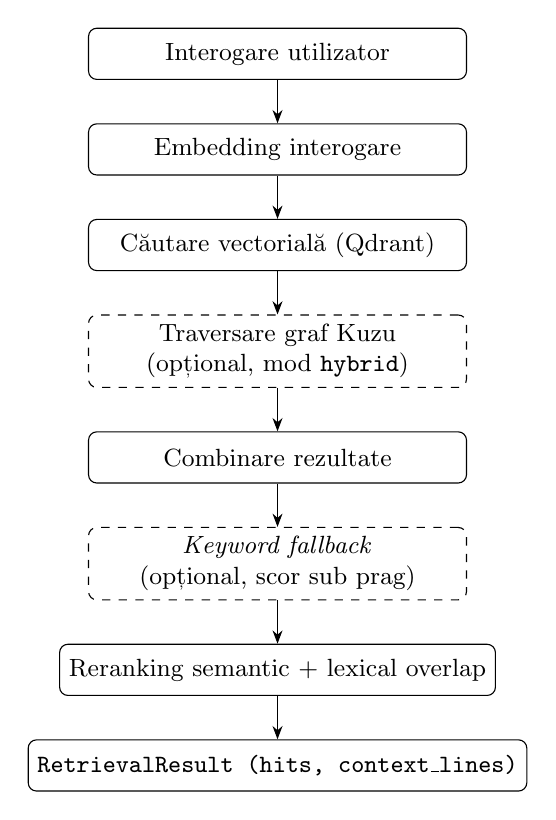
\begin{tikzpicture}[
  box/.style={draw, rounded corners=3pt, minimum width=4.8cm, minimum height=0.65cm, align=center, font=\small},
  opt/.style={draw, dashed, rounded corners=3pt, minimum width=4.8cm, minimum height=0.65cm, align=center, font=\small},
  >=Stealth, node distance=0.55cm
]
\node[box] (q)    {Interogare utilizator};
\node[box, below=of q]    (emb)  {Embedding interogare};
\node[box, below=of emb]  (vec)  {Căutare vectorială (Qdrant)};
\node[opt, below=of vec]  (gr)   {Traversare graf Kuzu\\(opțional, mod \texttt{hybrid})};
\node[box, below=of gr]   (merge){Combinare rezultate};
\node[opt, below=of merge](kw)   {\textit{Keyword fallback}\\(opțional, scor sub prag)};
\node[box, below=of kw]   (rr)   {Reranking semantic + lexical overlap};
\node[box, below=of rr]   (res)  {\texttt{RetrievalResult (hits, context\_lines)}};

\draw[->] (q)   -- (emb);
\draw[->] (emb) -- (vec);
\draw[->] (vec) -- (gr);
\draw[->] (gr)  -- (merge);
\draw[->] (merge) -- (kw);
\draw[->] (kw) -- (rr);
\draw[->] (rr) -- (res);
\end{tikzpicture}
\caption{Pipeline-ul de regăsire hibridă a contextului}
\label{fig:rag-retrieval}
\end{figure}

Această abordare este utilă în special pentru întrebările care implică relații medicale între concepte, de exemplu între boli, simptome, tratamente sau diagnostice diferențiale. Regăsirea vectorială oferă flexibilitate în identificarea fragmentelor relevante, în timp ce graful de cunoștințe adaugă o structură explicită a relațiilor dintre entități. Prin combinarea celor două surse de informație, sistemul poate construi un context mai bine fundamentat pentru generarea răspunsului.

\subsection{Extracția entităților și construirea grafului de cunoștințe}

Popularea grafului de cunoștințe se realizează prin extracția automată a entităților din documentele medicale utilizate. Modulul \texttt{knowledge/entities/extractor.py} folosește o abordare deterministă, bazată pe reguli, liste de termeni medicali și aliasuri normalizate, pentru identificarea entităților relevante. Entitățile extrase sunt filtrate pe baza unui prag de încredere și structurate conform schemei predefinite a grafului.

Entitățile sunt normalizate și deduplicate, iar noile înregistrări sunt fuzionate cu nodurile existente atunci când sunt detectate corespondențe. Astfel, se evită fragmentarea aceluiași concept medical în mai multe noduri distincte. Această abordare permite construirea incrementală a grafului pe măsura ingestiei de noi documente.

Graful de cunoștințe al proiectului este structurat în jurul a două tipuri principale de noduri: \texttt{Entity}, care reprezintă concepte medicale precum boli, simptome, medicamente sau structuri anatomice, și \texttt{SourceChunk}, care reprezintă fragmentele de document sursă. Relațiile principale utilizate sunt \texttt{MENTIONED\_IN}, \texttt{DISEASE\_HAS\_SYMPTOM}, \texttt{CONDITION\_CAUSES\_SYMPTOM}, \texttt{DRUG\_TREATS\_DISEASE} și \texttt{DISEASE\_DIFFERS\_FROM\_DISEASE}. Fiecare muchie reține metadate precum scorul de încredere, sursa, pagina și identificatorul fragmentului.

Detectarea relațiilor se realizează prin expresii trigger identificate în text, pe baza cărora sistemul stabilește legături între entități. De exemplu, o formulare care indică faptul că o boală este asociată cu un anumit simptom poate conduce la crearea unei relații de tip \texttt{DISEASE\_HAS\_SYMPTOM}. În mod similar, menționarea unei entități într-un fragment de document determină crearea unei relații de tip \texttt{MENTIONED\_IN} între nodul entitate și nodul corespunzător fragmentului sursă.

Pentru inspectarea grafului, baza de date Kuzu poate fi vizualizată cu ajutorul Kuzu Explorer. Deoarece Kuzu este utilizat ca bază de date embedded, datele sunt stocate local într-un director al proiectului, iar același director poate fi montat într-un container Docker care rulează interfața de vizualizare.

După pornirea containerului, interfața poate fi accesată în browser la adresa:

\begin{lstlisting}
http://localhost:8000
\end{lstlisting}

În această interfață pot fi rulate interogări Cypher pentru verificarea nodurilor și relațiilor existente. De exemplu:

\begin{lstlisting}[language=SQL]
MATCH (a)-[r]->(b)
RETURN a, r, b
LIMIT 5;
\end{lstlisting}

Rezultatul poate fi afișat atât tabelar, cât și sub formă de graf, unde nodurile sunt reprezentate prin cercuri, iar relațiile prin săgeți etichetate cu tipul relației. Această etapă nu este necesară pentru funcționarea sistemului în regim normal, dar este utilă pentru testare, depanare și validarea modului în care informațiile sunt organizate în baza de date grafică.


\subsection{Regăsirea hibridă vector-graf}

În modul hibrid, contextul furnizat modelului LLM este construit prin combinarea rezultatelor vectoriale cu informațiile obținute din traversarea grafului de cunoștințe. Pentru o interogare dată, sistemul identifică mai întâi fragmentele de text relevante prin similaritate vectorială, extrage entitățile medicale menționate în interogare, interogează graful pentru relațiile asociate acestor entități și concatenează toate informațiile recuperate într-un context unificat.

Această abordare crește relevanța răspunsului în cazul întrebărilor cu dependențe semantice complexe, permițând modelului să beneficieze atât de flexibilitatea regăsirii vectoriale, cât și de structura explicită a relațiilor codificate în graf.

\section{Modulul de evaluare}
\label{sec:evaluare}

Modulul de evaluare are rolul de a determina dacă un răspuns generat de modelul LLM este suficient de bun pentru a fi livrat utilizatorului. Implementat în pachetul \texttt{agent/evaluation}, acesta combină o etapă deterministă bazată pe euristici cu o etapă opțională asistată de un model LLM secundar, numit \textit{judecător} (\textit{LLM-as-a-judge}). Rezultatul evaluării este utilizat de motorul de raționament pentru a decide dacă răspunsul este acceptat sau dacă se impune o reluare cu un prompt adaptat sau cu un furnizor diferit.

\subsection{Arhitectura modulului}

Modulul este organizat în patru componente principale: \texttt{evaluator.py} — punctul de intrare care orchestrează evaluarea; \texttt{heuristics.py} — colecția de verificări deterministe; \texttt{failure\_taxonomy.py} — taxonomia tipurilor de eșec; \texttt{adaptive\_prompt.py} — generatorul de prompturi de reluare adaptate tipului de eșec; și \texttt{llm\_judge.py} — utilitarele pentru scenariul de arbitraj LLM. Configurația numerică (praguri, număr de reluări, ordine de fallback) este centralizată în \texttt{config/eval\_config.py} și poate fi suprascrisă prin variabile de mediu.

\subsection{Evaluarea euristică}

Prima etapă a evaluării constă în aplicarea unui set de verificări deterministe implementate în funcția \texttt{run\_heuristics}. Fiecărei verificări îi este asociată o penalizare numerică ce se scade dintr-un scor inițial de 1,0. Verificările sunt aplicate în ordine, iar scorul rezultat este trunchiat la 0,0 în cazul penalizărilor cumulate.

\begin{itemize}
    \item \textbf{Răspuns gol} (\texttt{EMPTY}): dacă răspunsul este complet absent, se aplică o penalizare maximă de 1,0, iar evaluarea se oprește imediat.
    \item \textbf{Răspuns prea scurt} (\texttt{TOO\_SHORT}): răspunsurile cu mai puțin de 10 caractere primesc o penalizare de 0,6.
    \item \textbf{Refuz în prezența contextului} (\texttt{REFUSED\_WITH\_CONTEXT}): dacă răspunsul conține fraze de tipul \textit{„nu știu"} sau \textit{„nu pot răspunde"} deși există fragmente de context recuperat, se aplică o penalizare de 0,45.
    \item \textbf{Răspuns incomplet} (\texttt{INCOMPLETE}): se penalizează cu 0,25 dacă lungimea răspunsului este sub pragul minim configurat (\texttt{safe\_min\_length}, implicit 80 de caractere) în prezența contextului; cu 0,2 dacă textul nu se termină cu semn de punctuație final.
    \item \textbf{Sfaturi medicale nesigure} (\texttt{UNSAFE\_ADVICE}): dacă răspunsul conține mențiuni de doze concrete (expresii numerice de tipul \textit{„500mg"}, \textit{„2 tablets"}) fără un avertisment de consultare a unui medic, penalizarea este de 0,5.
    \item \textbf{Ignorarea contextului} (\texttt{CONTEXT\_IGNORED}): se verifică suprapunerea lexicală dintre tokenii răspunsului și cei ai fragmentelor recuperate. O suprapunere sub 6\% semnalează că răspunsul nu utilizează contextul disponibil, cu o penalizare de 0,25.
    \item \textbf{Risc de halucinație} (\texttt{HALLUCINATION\_RISK}): dacă ignorarea contextului este însoțită de un răspuns lung, lipsit de formule de hedging și fără recomandare de consultare medicală, riscul de halucinație crește, penalizarea suplimentară fiind de 0,5.
    \item \textbf{Răspuns în afara subiectului} (\texttt{OFF\_TOPIC}): suprapunerea lexicală între tokenii interogării și cei ai răspunsului sub 5\% atrage o penalizare de 0,2.
\end{itemize}

\subsection{Arbitrajul LLM-as-a-judge}

Alegerea unui evaluator bazat în principal pe euristici deterministe, cu judecătorul LLM ca mecanism de arbitraj opțional, este motivată de compromisul latență-acuratețe. Un evaluator pur LLM ar adăuga un apel suplimentar de inferență la fiecare răspuns generat, dublând latența percepută de utilizator în cazul tipic în care răspunsul este corect. Euristica detectează direct cazurile extreme — gol, prea scurt, doze fără avertisment, ignorare completă a contextului — fără niciun cost de inferență. Judecătorul LLM este invocat exclusiv pentru zona de frontieră, unde decizia deterministă este nesigură, limitând astfel costul suplimentar la cazurile cu adevărat ambigue.

Dacă scorul euristic se situează în zona de frontieră definită de intervalul \texttt{[borderline\_low, borderline\_high]} (implicit [0,45; 0,65]) și funcția de judecată LLM este activată, evaluatorul apelează un model secundar pentru arbitraj. Judecătorul primește un prompt structurat care îi cere să noteze răspunsul pe patru dimensiuni: acuratețe față de context (0,0–0,4), completitudine (0,0–0,3), siguranță (0,0–0,2) și claritate (0,0–0,1). Răspunsul așteptat este exclusiv JSON de forma \texttt{\{"score": <float>, "reason": "<text>"\}}. Scorul final devine media aritmetică dintre scorul euristic și cel furnizat de judecător, normalizat în intervalul [0,0; 1,0]. Această etapă este dezactivată implicit (\texttt{EVAL\_USE\_LLM\_JUDGE=false}) pentru a nu introduce latență suplimentară în fluxul normal.

\subsection{Decizia de acceptare și strategia de reluare}

Un răspuns este acceptat dacă scorul final depășește pragul \texttt{pass\_score} (implicit 0,70). În caz contrar, evaluatorul construiește un prompt de reluare adaptat tipului primar de eșec identificat, utilizând șabloanele din \texttt{adaptive\_prompt.py}. Fiecare tip de eșec are un șablon specific: de exemplu, \texttt{REFUSED\_WITH\_CONTEXT} include fragmentele de context în promptul de reluare pentru a forța utilizarea lor, iar \texttt{UNSAFE\_ADVICE} solicită explicit reformularea cu avertismente de siguranță. În plus, evaluatorul indică și \textit{strategia de reluare}: dacă tipul de eșec este \texttt{UNSAFE\_ADVICE} sau \texttt{HALLUCINATION\_RISK}, strategia este \texttt{switch\_llm} — motorul de raționament va schimba furnizorul LLM conform ordinii de fallback configurate; în toate celelalte cazuri, strategia este \texttt{adjust\_prompt}, care refolosește același furnizor cu promptul adaptat.

\subsection{Structura rezultatului}

Evaluatorul returnează un obiect \texttt{EvaluatorResult} cu câmpurile: \texttt{passed} (boolean), \texttt{score} (float cu 4 zecimale), \texttt{reasons} (lista textelor asociate tipurilor de eșec), \texttt{failure\_types} (lista enumerărilor \texttt{FailureType}), \texttt{retry\_recommended} (boolean), \texttt{adaptive\_prompt} (promptul de reluare sau \texttt{None} dacă răspunsul a trecut), \texttt{retry\_strategy} (\texttt{"adjust\_prompt"} sau \texttt{"switch\_llm"}) și \texttt{judge\_used} (boolean care indică dacă arbitrajul LLM a fost invocat). Această structură permite motorului de raționament să ia decizii informate privind reluarea și permite urmărirea clară a procesului de evaluare a calității răspunsurilor.


\section{Interfața API a sistemului}

\subsection{Structura endpoint-urilor}

Interfața API este structurată în două categorii de endpoint-uri. Prima categorie cuprinde endpoint-uri interne dedicate fluxului aplicației, care includ operații de ingestie a documentelor, interogare conversațională și evaluare a calității răspunsului. A doua categorie cuprinde endpoint-uri compatibile cu formatul OpenAI Chat Completions API \cite{openai_api}, care permit utilizarea sistemului ca backend pentru orice client ce implementează protocolul OpenAI, fără modificări suplimentare la nivelul clientului. În această categorie sunt incluse endpoint-uri standard pentru interoperabilitate și operare, precum \texttt{/v1/chat/completions}, \texttt{/v1/models} și \texttt{/health}; pentru componenta de graf este expus și endpoint-ul \texttt{/graph/nexus}.

Această compatibilitate bidirecțională este esențială pentru integrarea cu OpenWebUI, un front-end open-source pentru interfețe conversaționale. Prin expunerea unui endpoint \texttt{/v1/chat/completions} conform specificației OpenAI, chatbot-ul medical poate fi accesat direct din OpenWebUI fără a necesita adaptări specifice de protocol.

\subsection{Securitatea interfaței}

Accesul la interfața API poate fi protejat printr-un mecanism de autentificare bazat pe chei API (\textit{API key authentication}), controlat prin variabila de mediu \texttt{API\_REQUIRE\_KEY}. Când această opțiune este activată, fiecare cerere trebuie să includă un token valid în header-ul HTTP (\texttt{Authorization: Bearer <API\_KEY>} sau \texttt{X-API-Key}), verificat de middleware înainte ca solicitarea să fie transmisă logicii aplicative. Această abordare reprezintă o practică standard de securitate pentru serviciile RESTful, protejând accesul la resurse sensibile și prevenind utilizarea neautorizată a serviciului \cite{flask_doc}.

Autentificarea este configurabilă prin variabile de mediu, putând fi 
activată sau dezactivată în funcție de contextul de deployment: 
dezactivată în mediul de dezvoltare locală și activă în orice 
configurație expusă extern.


\chapter{Interpretarea rezultatelor}

\section{Arhitectura propusă}

Modulul de benchmark --- implementat în \texttt{agent/benchmarking/benchmark.py} --- este distinct față de modulul de evaluare prezentat în secțiunea~\ref{sec:evaluare}. Modulul de evaluare face parte din pipeline-ul de răspuns al sistemului și validează calitatea unui singur răspuns generat în timp real. Modulul de benchmark operează în afara acestui flux: rulează un set standardizat de întrebări pe mai multe modele LLM simultan, în condiții identice, cu scopul de a produce metrici comparabile între configurații diferite. 


\subsection{Parsarea și normalizarea datelor}

Agentul pornește de la două surse de intrare: setul de întrebări de tip grilă în format JSON și cheia de răspuns asociată. Grilele medicale din dataset prezintă variații semnificative de structură: unele marchează răspunsurile corecte ca șir de caractere simplu, altele ca listă de litere, iar altele prin marcaj boolean pe fiecare opțiune în parte.

Pentru a gestiona aceste variații în mod uniform, etapa de încărcare normalizează fiecare item la schema internă \texttt{\{id, intrebare, choices\}}, cu opțiuni A--E uniforme și identificatori strict numerici. Același tratament se aplică și cheii de răspuns, normalizată la maparea \texttt{id -> set de litere}. Această normalizare este esențială deoarece permite o evaluare \textit{set-based} în locul uneia \textit{text-based}: compararea se face între mulțimi de litere, nu între șiruri de caractere, ceea ce elimină erorile cauzate de variații minore de formatare în răspunsul modelului (spații suplimentare, majuscule inconsistente, virgule sau paranteze extra).

\subsection{Detectarea tipului de grilă și generarea prompturilor}

Un aspect critic pentru corectitudinea benchmark-ului este tratarea neuniformității tipurilor de grilă medicală. Unele întrebări cer un singur răspuns corect, altele cer identificarea mai multor variante corecte simultan, iar tipul nu este întotdeauna explicit formulat în enunț.

Agentul detectează euristic această distincție combinând două surse de semnal: indicatori lexicali din textul întrebării (de exemplu, prezența sintagmelor specifice tipului de grilă) și tiparul structurii opțiunilor (secvențe de enunțuri independente față de combinații de opțiuni primare). Pe baza clasificării obținute, se generează prompturi distincte pentru fiecare categorie de grilă: \texttt{R.I.}, \texttt{u.a.s.c.c.e.}, \texttt{u.f.d.f.d.}, \texttt{c.e.} și \texttt{s.c.f.c.e.}



Fiecare prompt impune câmpuri de ieșire obligatorii adaptate tipului de grilă. Pentru întrebările de tip \textbf{R.I.} și \textbf{u.a.s.c.c.e.}, câmpurile obligatorii sunt \texttt{STATUS\_A} până la \texttt{STATUS\_E} (cu valorile \texttt{ADEVARAT} sau \texttt{FALS}) și \texttt{ANSWER} (literele finale selectate):

\begin{verbatim}
STATUS_A: ADEVARAT
STATUS_B: FALS
STATUS_C: ADEVARAT
STATUS_D: FALS
STATUS_E: FALS
ANSWER: A, C
\end{verbatim}

La tipul \textbf{u.a.s.c.c.e.}, răspunsul final este format din literele marcate cu \texttt{FALS}. La tipul \textbf{C.d.d.} (alegere unică), structura este identică, dar \texttt{ANSWER} conține o singură literă:

\begin{verbatim}
STATUS_A: INSUFICIENT
STATUS_B: FALS
STATUS_C: FALS
STATUS_D: ADEVARAT
STATUS_E: FALS
ANSWER: D
\end{verbatim}

Pentru întrebările de tip \textbf{F.d.u.} / \textbf{F.d.d.} (secvență temporală), modelul reconstruiește ordinea din context și o mapează la una dintre variantele A--E:

\begin{verbatim}
ORDER: e-c-a-b-d
OPTION: E
ANSWER: E
\end{verbatim}

Pentru întrebările cu \textbf{asocieri} (mapping între două coloane), câmpul \texttt{ASSOCIATIONS} conține perechile identificate, urmate de varianta selectată:

\begin{verbatim}
ASSOCIATIONS: a-2, b-1, c-3
OPTION: C
ANSWER: C
\end{verbatim}

Pentru întrebările de tip \textbf{s.c.f.c.e.} (construire frază), modelul generează fraza completă în câmpul \texttt{FRAZA}, identifică fragmentul problematic în \texttt{ISSUE\_FRAGMENT}, iar \texttt{ANSWER} conține litera corespunzătoare:

\begin{verbatim}
FRAZA: Procesele fiziologice prin care caldura este conservata
       (vasodilatatie) sau produsa (termogeneza musculara) continua
       pana cand temperatura sangelui care iriga neuronii
       hipotalamici corespunde noului nivel de referinta al
       termostatului
ISSUE_FRAGMENT: D
ANSWER: D
\end{verbatim}

Justificarea deciziei nu este extrasă ca un câmp separat, ci rezultă implicit din valorile \texttt{STATUS\_A--E}, a căror coerență internă este verificată în etapa de validare. Această structurare per tip de grilă are rolul de a forța consistența deciziei modelului și de a reduce ambiguitatea în etapa ulterioară de extragere a răspunsului final.
\subsection{Strategia de retrieval RAG}

Integrarea cu componenta RAG a necesitat o strategie de retrieval mai elaborată față de un simplu query cu textul întrebării. O singură interogare s-a dovedit insuficientă în cazul întrebărilor cu logică combinatorie, unde contextul relevant este distribuit în fragmente distincte din corpus --- de exemplu, când fiecare opțiune face referire la un concept sau situație clinică diferită.

Soluția adoptată construiește un \textit{pool de interogări} pentru fiecare grilă: întrebarea de bază plus câte o interogare pentru fiecare opțiune în parte, sub forma \texttt{Intrebare + Opțiunea X}. Rezultatele obținute din aceste interogări paralele sunt agregate și supuse unui proces de reranking cu scor compozit, care combină trei componente: scorul semantic inițial returnat de modelul de retrieval, overlap de tokeni cu textul întrebării și semnale de potrivire cu conținutul specific al fiecărei opțiuni. După reranking se aplică deduplicare la nivel de chunk, iar top-\textit{k} rezultate sunt concatenate ca și context final transmis modelului de inferență.

\subsection{Inferența și validarea răspunsurilor}

Pe partea de inferență, agentul utilizează un \textit{system prompt} conservator, orientat pe dovezi contextuale explicite. Modelului i se cere să răspundă exclusiv pe baza contextului recuperat, iar utilizarea cunoștințelor externe este descurajată explicit, pentru a evalua calitatea \textit{retrieval-ului} și nu memoria modelului.

Ieșirea este validată în două etape. Validarea structurală verifică prezența câmpurilor cerute și coerența dintre câmpul final și câmpurile intermediare, în funcție de tipul itemului: pentru întrebările cu răspuns unic, concordanța dintre \texttt{ANSWER} și statusurile individuale; pentru itemii de secvență, asociere și completare de fragment, concordanța dintre \texttt{ANSWER} și câmpurile dedicate precum \texttt{ORDER}, \texttt{ASSOCIATIONS} sau \texttt{ISSUE\_FRAGMENT}. Validarea semantică verifică dacă literele finale derivă corect din statusurile individuale și respinge răspunsurile care introduc raționament neancorat în context sau formulări speculative.

Răspunsurile care nu trec validarea sunt reluate cu un mesaj de revizuire. Pentru itemii cu răspuns unic există și un \textit{repair prompt} suplimentar, care impune explicit alegerea unei singure litere atunci când modelul returnează mai multe.
\subsection{Raportarea rezultatelor}

Rezultatul final al modulului este un raport structurat pe două niveluri de granularitate. La nivel de item se salvează: răspunsul brut al modelului, literele prezise, literele gold din cheia de răspuns, motivele de respingere (dacă există) și chunk-urile recuperate prin RAG. Această granularitate permite diagnosticarea erorilor individuale --- de retrieval, de formatare sau de raționament.

La nivel agregat se calculează metrici \textit{macro} --- \texttt{precision}, \texttt{recall} și \texttt{F1} mediate pe item --- și metrici \textit{micro} --- calculate din totalul cumulat al valorilor \texttt{tp}, \texttt{fp} și \texttt{fn} --- împreună cu \texttt{exact\_match\_rate} (proporția itemilor pentru care predicția coincide exact cu gold) și \texttt{global\_score}. Prin această structură, modulul devine nu doar un instrument de notare automată, ci o componentă de diagnostic al comportamentului sistemului LLM-RAG, utilă pentru identificarea și izolarea surselor de eroare pe fiecare etapă a pipeline-ului.

\section{Metrici de evaluare}

Evaluarea performanței unui model pe setul de întrebări de tip grilă nu poate fi redusă la o singură cifră, deoarece întrebările medicale admit atât răspunsuri unice, cât și răspunsuri multiple. Din această cauză, modulul calculează un set complet de metrici, grupate în trei categorii: metrici \textit{per item} (la nivel de întrebare individuală), metrici \textit{macro} (agregate prin mediere pe itemi) și metrici \textit{micro} (agregate prin cumularea erorilor la nivel global).

\subsection{Concepte de bază: TP, FP, FN}

Toate metricile derivă din trei valori fundamentale, calculate prin compararea mulțimii de litere prezise de model (\texttt{predicted}) cu mulțimea de litere corecte din cheia de răspuns (\texttt{gold}):

\begin{itemize}
    \item \textbf{True Positives (TP)} --- litere prezise corect, adică prezente atât în \texttt{predicted}, cât și în \texttt{gold}:
    \[ TP = |\texttt{predicted} \cap \texttt{gold}| \]

    \item \textbf{False Positives (FP)} --- litere prezise incorect, adică prezente în \texttt{predicted}, dar absente din \texttt{gold}:
    \[ FP = |\texttt{predicted} \setminus \texttt{gold}| \]

    \item \textbf{False Negatives (FN)} --- litere corecte omise, adică prezente în \texttt{gold}, dar absente din \texttt{predicted}:
    \[ FN = |\texttt{gold} \setminus \texttt{predicted}| \]
\end{itemize}

De exemplu, dacă răspunsul corect este $\{A, C, D\}$ și modelul prezice $\{A, B, D\}$, atunci $TP = 2$ (A și D), $FP = 1$ (B, prezis greșit) și $FN = 1$ (C, omis).

\subsection{Precision, Recall și F1 per item}

Pe baza valorilor TP, FP și FN, se calculează pentru fiecare item în parte:

\begin{itemize}
    \item \textbf{Precision} --- proporția răspunsurilor prezise care sunt corecte:
    \[ \text{precision}_i = \frac{TP_i}{TP_i + FP_i} \]
    O valoare ridicată indică faptul că modelul nu adaugă litere greșite, chiar dacă omite unele corecte.

    \item \textbf{Recall} --- proporția răspunsurilor corecte care au fost identificate:
    \[ \text{recall}_i = \frac{TP_i}{TP_i + FN_i} \]
    O valoare ridicată indică faptul că modelul nu omite litere corecte, chiar dacă adaugă și unele greșite.

    \item \textbf{F1} --- media armonică dintre precision și recall, care penalizează dezechilibrele între cele două:
    \[ F1_i = \frac{2 \cdot \text{precision}_i \cdot \text{recall}_i}{\text{precision}_i + \text{recall}_i} \]
    F1 este metrica principală per item, deoarece recompensează simultan acuratețea și completitudinea răspunsului.
\end{itemize}

Toate trei sunt definite ca $0$ când numitorul este $0$ (model fără nicio predicție sau item fără niciun răspuns corect în cheie).

\subsection{Metrici macro}

Metricile \textit{macro} se obțin prin medierea aritmetică a valorilor per grilă peste toate întrebările din set:

\[ \text{macro\_precision} = \frac{1}{N} \sum_{i=1}^{N} \text{precision}_i \]
\[ \text{macro\_recall} = \frac{1}{N} \sum_{i=1}^{N} \text{recall}_i \]
\[ \text{macro\_F1} = \frac{1}{N} \sum_{i=1}^{N} F1_i \]

unde $N$ este numărul total de itemi evaluați. Medierea macro tratează fiecare întrebare cu aceeași pondere, indiferent de numărul de răspunsuri corecte pe care îl conține. Aceasta înseamnă că o întrebare cu un singur răspuns corect și o întrebare cu patru răspunsuri corecte contribuie în mod egal la scorul final --- proprietate dezirabilă în contextul unui dataset cu distribuție neuniformă a tipurilor de grilă.

\subsection{Metrici micro}

Metricile \textit{micro} se calculează prin cumularea valorilor TP, FP și FN pentru toate grilele, înainte de a aplica formulele:

\[ \text{micro\_precision} = \frac{\sum_{i} TP_i}{\sum_{i} TP_i + \sum_{i} FP_i} \]
\[ \text{micro\_recall} = \frac{\sum_{i} TP_i}{\sum_{i} TP_i + \sum_{i} FN_i} \]
\[ \text{micro\_F1} = \frac{2 \cdot \text{micro\_precision} \cdot \text{micro\_recall}}{\text{micro\_precision} + \text{micro\_recall}} \]

Spre deosebire de metricile macro, varianta micro acordă implicit mai multă importanță întrebărilor cu mai multe răspunsuri corecte, deoarece acestea contribuie cu mai mulți TP/FP/FN la sumele cumulate. Compararea celor două variante oferă informații despre comportamentul modelului: o diferență mare între macro și micro F1 indică faptul că modelul performează neuniform în funcție de complexitatea întrebării (numărul de răspunsuri corecte).

\subsection{Exact Match Rate}

\texttt{exact\_match\_rate} măsoară proporția întrebărilor pentru care mulțimea prezisă coincide \textit{exact} cu mulțimea gold:

\[ \text{exact\_match\_rate} = \frac{|\{i : \texttt{predicted}_i = \texttt{gold}_i\}|}{N} \]

Această metrică este mai strictă decât F1: un item cu răspuns $\{A, C\}$ pentru care modelul prezice $\{A, B, C\}$ obține $F1 = 0.8$, dar contribuie cu $0$ la exact match rate. Exact match rate este relevantă în special pentru întrebările cu răspuns unic, unde orice abatere este o eroare completă, și constituie un indicator direct al ratei de răspuns corect în sens clasic de grilă.

\subsection{Global Score}

\texttt{global\_score} este o metrică sintetică obținută ca medie aritmetică între \texttt{macro\_F1} și \texttt{exact\_match\_rate}:

\[ \text{global\_score} = \frac{\text{macro\_F1} + \text{exact\_match\_rate}}{2} \]

Combinând cele două, scorul global recompensează atât răspunsurile parțial corecte (prin componenta F1), cât și acuratețea completă (prin componenta exact match). Un model care selectează întotdeauna un subset corect al răspunsurilor, fără a adăuga greșeli, va obține un F1 ridicat, dar un exact match scăzut --- global score penalizează acest comportament și favorizează modelele care identifică complet și precis mulțimea de răspunsuri corecte.
\section{Rezultatele obținute}

Evaluarea experimentală a fost realizată pe un set de 100 de întrebări medicale de tip grilă, cu cheie de răspuns completă. Pentru toate rulările prezentate în această secțiune au fost păstrate aceleași date de intrare, aceeași strategie de regăsire RAG și aceeași logică de parsare și validare a răspunsurilor. În acest fel, diferențele observate pot fi atribuite în principal comportamentului modelului lingvistic folosit pentru inferență. Rezultatele au fost extrase din rulările \texttt{output\_v33}--\texttt{output\_v37}, cu excluderea variantei locale Gemma, pentru a păstra comparația între modelele cloud evaluate în aceleași condiții de lucru.

\begin{table}[H]
\centering
\caption{Rezultatele comparative ale modelelor evaluate pe setul de 100 de grile}
\label{tab:rezultate_benchmark_llm}
\small
\setlength{\tabcolsep}{4pt}
\begin{tabular}{lcccccc}
\toprule
\textbf{Model} & \textbf{Global} & \textbf{Exact} & \textbf{Macro F1} & \textbf{Micro F1} & \textbf{Erori} & \textbf{Respingeri} \\
\midrule
GPT-5 mini & 0,9008 & 0,8900 & 0,9117 & 0,8991 & 11 & 4 \\
Claude Sonnet 4 & 0,8727 & 0,8600 & 0,8853 & 0,8826 & 14 & 10 \\
GPT-4o mini & 0,5047 & 0,4300 & 0,5793 & 0,5823 & 57 & 9 \\
GPT-5 & 0,9133 & 0,9000 & 0,9267 & 0,9252 & 10 & 2 \\
\bottomrule
\end{tabular}
\end{table}

Rezultatele indică o separare clară între modelele cu performanță ridicată și modelul \texttt{GPT-4o mini}. Cel mai bun rezultat global a fost obținut de \texttt{GPT-5}, cu un \texttt{global\_score} de 0,9133 și o rată de potrivire exactă de 90\%. Acest rezultat arată că modelul nu doar identifică frecvent literele corecte, ci reușește în majoritatea cazurilor să reproducă exact mulțimea de răspunsuri cerută de cheia de evaluare. Diferența dintre \texttt{macro\_F1} și \texttt{micro\_F1} este foarte redusă, ambele având valori apropiate de 0,925, ceea ce sugerează un comportament relativ stabil atât pentru întrebări cu răspuns unic, cât și pentru întrebări cu răspuns multiplu.

\texttt{GPT-5 mini} obține al doilea rezultat ca valoare globală, cu 0,9008 și 89\% exact match. Diferența față de \texttt{GPT-5} este mică, de 0,0125 la scorul global, ceea ce indică faptul că varianta mini păstrează o capacitate bună de urmărire a instrucțiunilor și de extragere a răspunsurilor din context. Totuși, valorile mai mici ale \texttt{micro\_precision} și \texttt{micro\_F1} arată că, în anumite cazuri, modelul introduce litere suplimentare sau omite parțial răspunsuri corecte în întrebările cu mai multe variante valide.

\texttt{Claude Sonnet 4} are un scor global de 0,8727 și o rată exact match de 86\%. Performanța este apropiată de cea a modelelor GPT mai puternice, dar numărul de respingeri structurale este mai mare: 10 răspunsuri au fost marcate cu motive precum \texttt{missing\_answer\_letters}, \texttt{status\_answer\_mismatch} sau \texttt{no\_derived\_answers}. Acest aspect arată că modelul poate ajunge la raționamente utile, dar are o tendință mai pronunțată de a produce ieșiri care nu respectă strict contractul de format cerut de benchmark. Într-un sistem automatizat, această diferență este importantă, deoarece un răspuns medical corect ca idee, dar greu de parsat sau inconsistent structural, nu poate fi evaluat sau livrat în mod fiabil fără mecanisme suplimentare de reparare.

Rezultatul obținut de \texttt{GPT-4o mini} este semnificativ mai slab: \texttt{global\_score} 0,5047, exact match 43\% și 57 de itemi fără potrivire exactă. Valorile \texttt{macro\_F1} și \texttt{micro\_F1}, ambele în jurul pragului de 0,58, arată că modelul produce frecvent răspunsuri parțial corecte, dar insuficient de precise pentru o evaluare strictă de tip grilă. Diferența dintre exact match și F1 sugerează că modelul identifică uneori o parte din răspunsul corect, însă adaugă litere incorecte sau omite variante relevante. Pentru aplicația propusă, acest comportament este problematic: în context medical, o predicție parțial corectă nu este echivalentă cu o soluție acceptabilă, deoarece opțiunile suplimentare sau omise pot schimba interpretarea clinică a răspunsului.

\subsection{Analiza erorilor}

Analiza răspunsurilor incorecte arată trei categorii principale de erori. Prima categorie este reprezentată de erorile de acoperire, în care modelul identifică doar o parte din mulțimea corectă. Exemplele de acest tip apar atunci când răspunsul corect conține două litere, dar modelul selectează doar una dintre ele. În aceste situații, \texttt{precision} rămâne ridicată, deoarece nu sunt introduse răspunsuri greșite, însă \texttt{recall} scade. Acest tip de eroare este vizibil în rulările modelelor \texttt{GPT-5 mini} și \texttt{GPT-5}, unde unele întrebări cu răspuns multiplu sunt rezolvate incomplet.

A doua categorie este reprezentată de supraselecție, în care modelul include litere suplimentare față de cheia corectă. Aceasta afectează direct \texttt{precision} și exact match. Cazurile în care modelul returnează mai multe variante decât cele acceptate arată o dificultate de separare între afirmațiile susținute explicit de context și afirmațiile plauzibile, dar neconfirmate suficient. Această problemă este mai evidentă la \texttt{GPT-4o mini}, unde numeroase predicții conțin combinații de litere care includ parțial răspunsul corect, dar adaugă și opțiuni greșite.

A treia categorie este formată din erori structurale de ieșire. Acestea includ situații în care câmpul \texttt{ANSWER} lipsește, literele nu pot fi extrase, sau există contradicții între statusurile intermediare și răspunsul final. Numărul acestor respingeri este cel mai mic pentru \texttt{GPT-5}, cu doar 2 cazuri, și cel mai mare pentru \texttt{Claude Sonnet 4}, cu 10 cazuri. Această observație confirmă importanța validării structurale: benchmark-ul nu măsoară doar cunoștințele modelului, ci și capacitatea lui de a respecta un protocol formal de răspuns, condiție necesară pentru integrarea într-un sistem software reproductibil.

\subsection{Interpretarea comparativă}

Din perspectiva calității finale, \texttt{GPT-5} este modelul cel mai potrivit pentru configurația evaluată, deoarece combină cel mai mare scor global cu cel mai mic număr de respingeri structurale. Acest lucru indică atât o capacitate mai bună de raționament pe contextul recuperat, cât și o conformare mai bună la formatul impus de agentul de benchmark. \texttt{GPT-5 mini} reprezintă o alternativă apropiată, cu o scădere modestă de performanță, ceea ce îl face relevant în scenarii în care costul sau latența sunt constrângeri importante.

\texttt{Claude Sonnet 4} obține rezultate competitive ca scor, dar necesită o atenție mai mare asupra constrângerilor de format. Într-o integrare practică, acest model ar beneficia de prompturi mai restrictive sau de un pas suplimentar de normalizare a ieșirii. În schimb, \texttt{GPT-4o mini} nu oferă performanță suficientă pentru sarcina evaluată în forma curentă. Deși poate produce răspunsuri parțiale utile, rata mare de erori exacte îl face nepotrivit ca model principal pentru un agent medical bazat pe grile, unde evaluarea depinde de identificarea completă a variantelor corecte.

În ansamblu, rezultatele susțin utilitatea arhitecturii propuse. Strategia de retrieval și validare permite compararea coerentă a modelelor și evidențiază diferențe care nu ar fi vizibile printr-o simplă inspecție manuală a răspunsurilor. În același timp, evaluarea arată că performanța finală nu depinde exclusiv de calitatea contextului recuperat, ci și de disciplina modelului în respectarea formatului, de capacitatea de a distinge între răspunsuri susținute și răspunsuri plauzibile și de robustețea la întrebări cu structură combinatorie.
\chapter{Concluzii}
\section{Concluzii generale}
Lucrarea evidențiază faptul că integrarea LLM cu RAG și cu un flux agentic de validare poate crește fiabilitatea răspunsurilor în domeniul medical, cu condiția utilizării unor surse bine curate și a unor mecanisme explicite de control al calității.

\section{Direcții viitoare}
Extinderile naturale includ optimizarea strategiei de recuperare a contextului, îmbunătățirea evaluatorului prin criterii mai fine și integrarea unui mecanism de citare automată a surselor în răspunsul final.

\bibliographystyle{unsrt}
\bibliography{referinte}

\appendix
\chapter{Fragmente relevante de cod}

Această anexă include fragmentele de cod considerate reprezentative pentru implementarea sistemului. Selecția nu urmărește reproducerea integrală a fișierelor sursă, ci evidențierea componentelor care susțin arhitectura descrisă în capitolele anterioare: orchestrarea cererii, regăsirea contextului, rutarea către modele LLM, evaluarea răspunsurilor și benchmark-ul comparativ.

\section{Orchestrarea fluxului principal}

Fragmentul următor prezintă metoda principală a orchestratorului. Aceasta aplică mai întâi regulile de protecție, iar în cazul unei cereri valide transferă controlul către motorul de raționament. Rezultatul final agregă răspunsul generat, furnizorul LLM utilizat, numărul de reluări, rezultatul evaluatorului și informațiile de retrieval.

\begin{lstlisting}[language=Python, caption={Fluxul principal al orchestratorului}]
def run(self, request: QueryRequest) -> OrchestratorResponse:
    """Run the full request lifecycle and return the final response."""

    guardrail_result = self._deps.guardrail(request.query)
    if not guardrail_result.is_valid:
        return OrchestratorResponse(
            response=guardrail_result.message,
            provider=None,
            model=None,
            retries=0,
            guardrail=guardrail_result,
            evaluator=None,
            retrieval=None,
            context_lines=[],
        )

    reasoning_result = self._reasoning_engine.run(
        ReasoningInput(
            query=request.query,
            top_k=request.top_k,
            language=request.language,
            filters=request.filters,
        )
    )

    return OrchestratorResponse(
        response=reasoning_result.response,
        provider=reasoning_result.provider,
        model=reasoning_result.model,
        retries=reasoning_result.retries,
        guardrail=guardrail_result,
        evaluator=reasoning_result.evaluator,
        retrieval=reasoning_result.retrieval,
        context_lines=reasoning_result.context_lines,
    )
\end{lstlisting}

\section{Motorul de raționament și mecanismul de reluare}

Motorul de raționament realizează legătura dintre retrieval, generare și evaluare. După recuperarea fragmentelor relevante, construiește promptul cu context și execută una sau mai multe încercări de generare. Dacă evaluatorul indică o problemă și recomandă reluarea, următoarea încercare primește instrucțiuni corective sau poate folosi un alt furnizor LLM.

\begin{lstlisting}[language=Python, caption={Bucla de generare, evaluare și retry}]
retrieval_result = self._deps.retrieve(
    request.query,
    request.top_k,
    retrieval_filters,
)

if not retrieval_result.hits or retrieval_result.max_score() < min_score:
    return ReasoningOutput(
        response=LOW_CONFIDENCE_MESSAGE,
        provider=None,
        model=None,
        retries=0,
        evaluator=None,
        retrieval=retrieval_result,
        context_lines=[],
    )

context_lines = retrieval_result.context_lines(with_score=True)
base_request = LLMRequest(
    system_prompt=self._system_prompt,
    user_message=request.query,
    context_block=build_context_block(context_lines),
)

for attempt in range(max_attempts):
    provider = self._select_provider(attempt, last_eval)
    attempt_request = self._apply_retry_guidance(base_request, last_eval)
    attempt_request.provider = provider

    last_response = self._deps.llm_call(attempt_request)
    last_eval = self._deps.evaluator(
        request.query,
        last_response.content,
        context_lines,
    )

    if last_eval.passed or not last_eval.retry_recommended:
        break
\end{lstlisting}

\section{Rutarea către furnizorii LLM}

Sistemul folosește o interfață unificată pentru furnizori diferiți. Funcția de rutare primește o cerere de tip \texttt{LLMRequest}, determină furnizorul configurat și returnează un obiect \texttt{LLMResponse} care conține atât textul generat, cât și metadatele despre provider și model.

\begin{lstlisting}[language=Python, caption={Rutarea unei cereri către providerul LLM configurat}]
def llm_ask_request(request: LLMRequest) -> LLMResponse:
    """Route an LLMRequest to the configured provider."""

    provider = _select_provider(request.provider)
    if provider == PROVIDER_OLLAMA:
        content = ollama_call(
            messages=request.messages(),
            temperature=request.temperature,
        )
        return LLMResponse(
            content=content,
            provider=PROVIDER_OLLAMA,
            model=SETTINGS.ollama_model,
        )

    if provider == PROVIDER_QWEN:
        content = qwen_call(
            messages=request.messages(),
            temperature=request.temperature,
        )
        return LLMResponse(content=content, provider=PROVIDER_QWEN,
                           model=SETTINGS.qwen_model)

    if provider == PROVIDER_ANTHROPIC:
        content = anthropic_call(
            messages=request.messages(),
            temperature=request.temperature,
        )
        return LLMResponse(content=content, provider=PROVIDER_ANTHROPIC,
                           model=SETTINGS.anthropic_model)

    content = openai_call(
        messages=request.messages(),
        temperature=request.temperature,
    )
    return LLMResponse(content=content, provider=PROVIDER_OPENAI,
                       model=SETTINGS.openai_model)
\end{lstlisting}

\section{Regăsirea contextului prin RAG}

Fragmentul următor prezintă funcția de intrare pentru retrieval. În funcție de configurație, sistemul poate folosi retrieval vectorial simplu sau retrieval hibrid. În modul vectorial, interogarea este transformată în embedding, sunt recuperate fragmente candidate din Qdrant, iar rezultatele pot fi rerankate înainte de a fi transmise modelului generativ.

\begin{lstlisting}[language=Python, caption={Funcția de intrare pentru retrieval vectorial sau hibrid}]
def retrieve_top_similar(
    input_message: str,
    top_k: int = 5,
    filter_by: dict[str, str] | None = None,
    *,
    retrieval_mode: str | None = None,
) -> RetrievalResult:
    """Dispatch retrieval in vector or hybrid mode."""

    filter_mode = None
    if filter_by:
        filter_mode = filter_by.get(_POLICY_RETRIEVAL_MODE_KEY)

    mode = (
        filter_mode or retrieval_mode or SETTINGS.retrieval_mode
    ).strip().lower()

    if mode == "hybrid":
        return retrieve_hybrid(input_message, top_k=top_k,
                               filter_by=filter_by)

    candidate_k = (
        max(top_k, SETTINGS.retrieval_rerank_top_k)
        if SETTINGS.retrieval_rerank_enabled
        else top_k
    )
    vector_hits = _vector_hits(input_message, top_k=candidate_k,
                               filter_by=filter_by)
    provenance = "vector"

    if SETTINGS.retrieval_rerank_enabled:
        vector_hits = _rerank_hits(input_message, vector_hits, top_k=top_k)
    else:
        vector_hits = vector_hits[:top_k]

    return RetrievalResult(hits=vector_hits, provenance=provenance)
\end{lstlisting}

\section{Reguli de protecție pentru cererile utilizatorilor}

Componenta de guardrails aplică o strategie deterministă înaintea apelului către LLM. Sunt verificate mai întâi cazurile cu risc ridicat, precum urgențele medicale și cererile nesigure. Numai cererile validate ajung în etapa de retrieval și generare.

\begin{lstlisting}[language=Python, caption={Aplicarea regulilor deterministe de guardrail}]
def apply_guardrails(query: str) -> GuardrailResult:
    """Evaluate user query safety."""

    if not query or not query.strip():
        result = _base_result(
            category=CATEGORY_AMBIGUOUS,
            reason_code=REASON_EMPTY_QUERY,
            confidence=CONFIDENCE_EMPTY,
            is_valid=False,
        )
        result.message = EMPTY_QUERY_MESSAGE
        return result

    normalized_query = normalize_query(query)

    emergency_matches = find_grouped_matches(
        normalized_query,
        EMERGENCY_PATTERN_GROUPS,
    )
    if emergency_matches and not _is_educational_context(normalized_query):
        result = _base_result(
            category=CATEGORY_EMERGENCY,
            reason_code=REASON_KEYWORD_EMERGENCY,
            confidence=CONFIDENCE_KEYWORD_HIGH_RISK,
            is_valid=False,
        )
        result.is_emergency = True
        result.message = EMERGENCY_MESSAGE
        result.matched_keywords = emergency_matches
        return result

    critical_unsafe_matches = find_grouped_matches(
        normalized_query,
        UNSAFE_CRITICAL_PATTERN_GROUPS,
    )
    if critical_unsafe_matches:
        result = _base_result(
            category=CATEGORY_UNSAFE,
            reason_code=REASON_KEYWORD_UNSAFE_CRITICAL,
            confidence=CONFIDENCE_KEYWORD_HIGH_RISK,
            is_valid=False,
        )
        result.is_unsafe = True
        result.message = UNSAFE_CRITICAL_MESSAGE
        result.matched_keywords = critical_unsafe_matches
        return result
\end{lstlisting}

\section{Evaluarea răspunsurilor generate}

Evaluatorul transformă verificările euristice într-un scor numeric și într-o decizie de acceptare sau respingere. Dacă răspunsul nu trece pragul minim, este construit un prompt adaptiv de reluare, iar pentru anumite tipuri de eșec strategia poate deveni schimbarea modelului LLM.

\begin{lstlisting}[language=Python, caption={Calculul scorului și alegerea strategiei de retry}]
def evaluate_response(
    query: str,
    response: str,
    context_lines: list[str] | None = None,
    use_llm_judge: bool | None = None,
    llm_judge_fn=None,
) -> EvaluatorResult:
    """Evaluate whether an answer is acceptable."""

    context_lines = context_lines or []
    issues = run_heuristics(query, response, context_lines)

    score = 1.0
    failure_types: list[FailureType] = []
    reasons: list[str] = []
    for failure_type, penalty in issues:
        score -= penalty
        failure_types.append(failure_type)
        reasons.append(failure_type.value)
    score = max(score, 0.0)

    passed = score >= EVAL_CONFIG.pass_score

    adaptive_prompt: str | None = None
    retry_strategy = "adjust_prompt"
    if not passed:
        primary_failure = failure_types[0] if failure_types else UNKNOWN_FAILURE
        adaptive_prompt = build_adaptive_prompt(
            failure_type=primary_failure,
            query=query,
            bad_response=response,
            context_lines=context_lines,
        )
        if any(failure in SWITCH_LLM_FAILURES
               for failure in failure_types):
            retry_strategy = "switch_llm"

    return EvaluatorResult(
        passed=passed,
        score=round(score, 4),
        reasons=reasons,
        retry_recommended=not passed,
        failure_types=failure_types,
        adaptive_prompt=adaptive_prompt,
        retry_strategy=retry_strategy,
    )
\end{lstlisting}

\section{Benchmark-ul pentru întrebări de tip grilă}

Pentru evaluarea comparativă, benchmark-ul construiește un pool de interogări pentru fiecare item: întrebarea de bază și câte o interogare pentru fiecare opțiune. Rezultatele sunt rerankate și deduplicate înainte de a forma contextul transmis modelului. Această strategie crește șansa ca fragmentele relevante pentru fiecare variantă de răspuns să fie incluse în prompt.

\begin{lstlisting}[language=Python, caption={Construirea pool-ului de interogări și rerankarea contextului}]
def _build_option_queries(item: dict[str, Any]) -> list[str]:
    """Build query pool containing base question and per-option probes."""

    question = item["intrebare"]
    queries = [question]
    for letter, value in item["choices"].items():
        cleaned = value.strip()
        if not cleaned:
            continue
        queries.append(f"{question}\nOptiunea {letter}: {cleaned}")
    return queries


def _rerank_benchmark_hits(
    item: dict[str, Any],
    hits: list[RetrievalHit],
    *,
    top_k: int,
) -> list[RetrievalHit]:
    """Rerank and deduplicate retrieval hits."""

    weighted = sorted(
        ((_benchmark_hit_relevance(item, hit), hit) for hit in hits),
        key=lambda pair: pair[0],
        reverse=True,
    )
    deduped: list[RetrievalHit] = []
    seen: set[tuple[str | None, int | None, str | None, str]] = set()
    for _score, hit in weighted:
        key = (hit.source_file, hit.page, hit.chunk_id, hit.text)
        if key in seen:
            continue
        seen.add(key)
        deduped.append(hit)
        if len(deduped) >= top_k:
            break
    return deduped
\end{lstlisting}

Metricile finale sunt calculate prin compararea mulțimii de litere prezise cu mulțimea de litere din cheia de răspuns. Acest mod de evaluare este adecvat pentru grile cu răspuns unic și multiplu, deoarece penalizează atât variantele greșit adăugate, cât și variantele corecte omise.

\begin{lstlisting}[language=Python, caption={Calculul metricilor per item pentru benchmark}]
def _score_prediction(
    predicted: set[str],
    gold: set[str],
) -> dict[str, float | int | bool]:
    """Compute per-item set metrics for benchmark answers."""

    true_positive = len(predicted & gold)
    false_positive = len(predicted - gold)
    false_negative = len(gold - predicted)

    precision = true_positive / len(predicted) if predicted else 0.0
    recall = true_positive / len(gold) if gold else 1.0
    f1 = (
        2 * precision * recall / (precision + recall)
        if (precision + recall) > 0
        else 0.0
    )

    return {
        "tp": true_positive,
        "fp": false_positive,
        "fn": false_negative,
        "precision": round(precision, 4),
        "recall": round(recall, 4),
        "f1": round(f1, 4),
        "exact_match": predicted == gold,
    }
\end{lstlisting}

\end{document}
